        %%******************************************%%
        %%                                          %%
        %%        Modello di tesi di laurea         %%
        %%            di Andrea Giraldin            %%
        %%                                          %%
        %%             2 novembre 2012              %%
        %%                                          %%
        %%******************************************%%


% I seguenti commenti speciali impostano:
% 1. 
% 2. PDFLaTeX come motore di composizione;
% 3. tesi.tex come documento principale;
% 4. il controllo ortografico italiano per l'editor.

% !TEX encoding = UTF-8
% !TEX TS-program = pdflatex
% !TEX root = tesi.tex
% !TEX spellcheck = it-IT

\documentclass[10pt,                    % corpo del font principale
               a4paper,                 % carta A4
               twoside,                 % impagina per fronte-retro
               openright,               % inizio capitoli a destra
               english,                 
               italian,                 
               ]{book}    

\usepackage[utf8]{inputenc}             % codifica di input; anche [latin1] va bene
                                        % NOTA BENE! va accordata con le preferenze dell'editor

%**************************************************************
% Importazione package
%************************************************************** 

%\usepackage{amsmath,amssymb,amsthm}    % matematica

\usepackage[english, italian]{babel}    % per scrivere in italiano e in inglese;
                                        % l'ultima lingua (l'italiano) risulta predefinita

\usepackage{bookmark}                   % segnalibri

\usepackage{caption}                    % didascalie

\usepackage{chngpage,calc}              % centra il frontespizio

\usepackage{csquotes}                   % gestisce automaticamente i caratteri (")

\usepackage{emptypage}                  % pagine vuote senza testatina e piede di pagina

\usepackage{epigraph}					% per epigrafi

\usepackage{eurosym}                    % simbolo dell'euro

\usepackage[T1]{fontenc}                % codifica dei font:
                                        % NOTA BENE! richiede una distribuzione *completa* di LaTeX

%\usepackage{indentfirst}               % rientra il primo paragrafo di ogni sezione

\usepackage{graphicx}                   % immagini

\usepackage{hyperref}                   % collegamenti ipertestuali



\usepackage[binding=5mm]{layaureo}      % margini ottimizzati per l'A4; rilegatura di 5 mm

\usepackage{listings}                   % codici

\usepackage{microtype}                  % microtipografia

\usepackage{mparhack,fixltx2e,relsize}  % finezze tipografiche

\usepackage{nameref}                    % visualizza nome dei riferimenti                                      

\usepackage[font=small]{quoting}        % citazioni

\usepackage{subfig}                     % sottofigure, sottotabelle

\usepackage[italian]{varioref}          % riferimenti completi della pagina

\usepackage[dvipsnames]{xcolor}         % colori
\usepackage[section]{placeins}

\usepackage{booktabs}                   % tabelle                                       
\usepackage{tabularx}                   % tabelle di larghezza prefissata                                    
\usepackage{longtable}                  % tabelle su più pagine                                        
\usepackage{ltxtable}                   % tabelle su più pagine e adattabili in larghezza

\usepackage[toc, acronym]{glossaries}   % glossario
                                        % per includerlo nel documento bisogna:
                                        % 1. compilare una prima volta tesi.tex;
                                        % 2. eseguire: makeindex -s tesi.ist -t tesi.glg -o tesi.gls tesi.glo
                                        % 3. eseguire: makeindex -s tesi.ist -t tesi.alg -o tesi.acr tesi.acn
                                        % 4. compilare due volte tesi.tex.
\tolerance=1
\emergencystretch=\maxdimen
\hyphenpenalty=10000
\hbadness=10000
\usepackage[backend=biber,style=verbose-ibid,hyperref,backref]{biblatex}
                                        % eccellente pacchetto per la bibliografia; 
                                        % produce uno stile di citazione autore-anno; 
                                        % lo stile "numeric-comp" produce riferimenti numerici
                                        % per includerlo nel documento bisogna:
                                        % 1. compilare una prima volta tesi.tex;
                                        % 2. eseguire: biber tesi
                                        % 3. compilare ancora tesi.tex.

%**************************************************************
% file contenente le impostazioni della tesi
%**************************************************************

%**************************************************************
% Frontespizio
%**************************************************************
\newcommand{\myName}{Trevisan Davide} 													% autore
\newcommand{\myMatricola}{1070686}                               % matricola
\newcommand{\myTitle}{Sviluppo di un modulo in Alfresco, sistema di gestione della conoscenza }                    
\newcommand{\myDegree}{Tesi di laurea triennale}                % tipo di tesi
\newcommand{\myUni}{Università degli Studi di Padova}           % università
\newcommand{\myFaculty}{Corso di Laurea in Informatica}         % facoltà
\newcommand{\myDepartment}{Dipartimento di Matematica}          % dipartimento
\newcommand{\myProf}{Gaggi Ombretta}                                % relatore
\newcommand{\myLocation}{Padova}                                % dove
\newcommand{\myAA}{2016-2017}                                   % anno accademico
\newcommand{\myTime}{Aprile 2017}                                  % quando


%**************************************************************
% Impostazioni di impaginazione
% see: http://wwwcdf.pd.infn.it/AppuntiLinux/a2547.htm
%**************************************************************

\setlength{\parindent}{14pt}   % larghezza rientro della prima riga
\setlength{\parskip}{0pt}   % distanza tra i paragrafi


%**************************************************************
% Impostazioni di biblatex
%**************************************************************
\bibliography{bibliografia} % database di biblatex 

\defbibheading{bibliography}
{
    \cleardoublepage
    \phantomsection 
    \addcontentsline{toc}{chapter}{\bibname}
    \chapter*{\bibname\markboth{\bibname}{\bibname}}
}

\setlength\bibitemsep{1.5\itemsep} % spazio tra entry

\DeclareBibliographyCategory{opere}
\DeclareBibliographyCategory{web}

\addtocategory{opere}{womak:lean-thinking}
\addtocategory{web}{site:agile-manifesto}

\defbibheading{opere}{\section*{Riferimenti bibliografici}}
\defbibheading{web}{\section*{Siti Web consultati}}


%**************************************************************
% Impostazioni di caption
%**************************************************************
\captionsetup{
    tableposition=top,
    figureposition=bottom,
    font=small,
    format=hang,
    labelfont=bf
}

%**************************************************************
% Impostazioni di glossaries
%**************************************************************

%**************************************************************
% Acronimi
%**************************************************************
\renewcommand{\acronymname}{Acronimi e abbreviazioni}
\newacronym[description={\glslink{API}{Application Program Interface}}]
    {api}{API}{Application Program Interface}
\newacronym[description={\glslink{KMS}{Knowledge Managment System}}]
    {kms}{KMS}{Knowledge Managment System}
\newacronym[description={\glslink{ICT}{Information and Communication Tecnology}}]
    {ict}{ICT}{Information and Communication Tecnology}
\newacronym[description={\glslink{B2B}{Business-to-business}}]
    {b2b}{B2B}{Business-to-business}		
\newacronym[description={\glslink{B2C}{Business-to-Business}}]
    {b2c}{B2C}{Business-to-Consumer}		
\newacronym[description={\glslink{YUI}{Yahoo! User Interface Library}}]
    {yui}{YUI}{Yahoo! User Interface Library}

%**************************************************************
% Glossario
%**************************************************************
\renewcommand{\glossaryname}{Glossario}

\newglossaryentry{API}
{
    name=\glslink{api}{API},
    text=Application Program Interface,
    sort=api,
    description={in informatica con il termine \emph{Application Programming Interface API} (ing. interfaccia di programmazione di un'applicazione) si indica ogni insieme di procedure disponibili al programmatore, di solito raggruppate a formare un set di strumenti specifici per l'espletamento di un determinato compito all'interno di un certo programma. La finalità è ottenere un'astrazione, di solito tra l'hardware e il programmatore o tra software a basso e quello ad alto livello semplificando così il lavoro di programmazione}
}

%\newglossaryentry{umlg}
%{
    %name=\glslink{uml}{UML},
    %text=UML,
    %sort=uml,
    %description={in ingegneria del software \emph{UML, Unified Modeling Language} (ing. linguaggio di modellazione unificato) è un linguaggio di modellazione e specifica basato sul paradigma object-oriented. L'\emph{UML} svolge un'importantissima funzione di ``lingua franca'' nella comunità della progettazione e programmazione a oggetti. Gran parte della letteratura di settore usa tale linguaggio per descrivere soluzioni analitiche e progettuali in modo sintetico e comprensibile a un vasto pubblico}
%}
\newglossaryentry{KMS}{
    name=\glslink{kms}{KMS},
    text=KMS,
    sort=uml,
    description={Knowledge management system:\\
		I Knowledge management system sono sistemi software che supportano le fasi del ciclo dell'informazione e la comunicazione all'interno di una comunità di pratica (ad esempio un'azienda) o di apprendimento (ad esempio una classe "virtuale") anche disperse nello spazio. Dovrebbero assistere le persone ad esplicitare la conoscenza tacita, a reperirla, a condividerla, supportando in particolare le seguenti funzioni:
		\begin{itemize}
			\item Cattura delle competenze collettive
\item Controllo per realizzare obiettivi comuni
\item Integrazione delle conoscenze frammentate
		\end{itemize}
}
}
\newglossaryentry{ICT}{
    name=\glslink{ict}{ICT},
    text=ICT,
    sort=ict,
    description={Information and communication tecnology:\\ Le tecnologie dell'informazione e della comunicazione (in inglese Information and Communications Technology, in acronimo ICT), sono l'insieme dei metodi e delle tecnologie che realizzano i sistemi di trasmissione, ricezione ed elaborazione di informazioni (tecnologie digitali comprese)}
		}
\newglossaryentry{B2C}{
   name=\glslink{b2c}{B2C},
    text=B2C,
    sort=b2c,
    description={Con Business to Consumer, spesso abbreviato in \emph{B2C}, si indicano le relazioni che un'impresa commerciale detiene con i suoi clienti per le attività di vendita e/o di assistenza}
		}
\newglossaryentry{B2B}{
    name=\glslink{b2b}{B2B},
    text=B2B,
    sort=b2b,
    description={Business-to-business, spesso indicato con l'acronimo \emph{B2B}, in italiano commercio interaziendale, è una locuzione utilizzata per descrivere le transazioni commerciali elettroniche tra imprese, distinguendole da quelle che intercorrono tra le imprese e altri gruppi, come quelle oppure quelle tra una impresa e il governo}}
\newglossaryentry{YUI}{
    name=\glslink{yui}{YUI},
    text=YUI,
    sort=yui,
    description={YUI è una libreria open-source JavaScript per scrivere applicazioni web interattive usando tecniche come Ajax, DHTML, e scripting DOM. YUI include anche molte risorse CSS nel suo nucleo. È disponibile con licenza BSD.Lo sviluppo su YUI è iniziato nel 2005 e nell'estate di quell'anno iniziò il suo utilizzo sulle pagine di Yahoo!.È stato rilasciato per uso pubblico nel 2006.
Nel settembre 2009, Yahoo! ha rilasciato YUI 3, una versione ricostruita da zero apprendendo dagli errori commessi con YUI 2. Tra le caratteristiche più degne di nota vi è l'adozione di JQuery per la selezione degli elementi per il CSS.
Il 29 agosto 2014 è stato annunciato il termine dello sviluppo attivo, dovuto al calo di interesse per le grandi librerie JavaScript, alla evoluzione dello stesso JavaScript e al proliferare di soluzioni server-side. Gli sviluppi futuri si limiteranno alla sistemazione di bug ritenuti critici}}
\newglossaryentry{Activiti Workflow Engine}{
    name=Activiti Workflow Engine,
    text=Activiti Workflow Engine,
    sort=Activiti Workflow Engine,
    description={Activiti è un leggera piattaforma per workflow e BPM (Business Process Management). Il suo cuore è l'engine BPMN2 (Business Process Model and Notation) per Java. È open-source e distribuito attraverso licenzaApache. Activiti funziona in qualsiasi applicazione Java, su un server, su un cluster o nel cloud. Si integra con Spring, è estremamente leggero e basato su concetti semplici
}} % database di termini
\makeglossaries


%**************************************************************
% Impostazioni di graphicx
%**************************************************************
\graphicspath{{immagini/}} % cartella dove sono riposte le immagini


%**************************************************************
% Impostazioni di hyperref
%**************************************************************
\hypersetup{
    %hyperfootnotes=false,
    %pdfpagelabels,
    %draft,	% = elimina tutti i link (utile per stampe in bianco e nero)
    colorlinks=true,
    linktocpage=true,
    pdfstartpage=1,
    pdfstartview=FitV,
    % decommenta la riga seguente per avere link in nero (per esempio per la stampa in bianco e nero)
    %colorlinks=false, linktocpage=false, pdfborder={0 0 0}, pdfstartpage=1, pdfstartview=FitV,
    breaklinks=true,
    pdfpagemode=UseNone,
    pageanchor=true,
    pdfpagemode=UseOutlines,
    plainpages=false,
    bookmarksnumbered,
    bookmarksopen=true,
    bookmarksopenlevel=1,
    hypertexnames=true,
    pdfhighlight=/O,
    %nesting=true,
    %frenchlinks,
    urlcolor=webbrown,
    linkcolor=RoyalBlue,
    citecolor=webgreen,
    %pagecolor=RoyalBlue,
    %urlcolor=Black, linkcolor=Black, citecolor=Black, %pagecolor=Black,
    pdftitle={\myTitle},
    pdfauthor={\textcopyright\ \myName, \myUni, \myFaculty},
    pdfsubject={},
    pdfkeywords={},
    pdfcreator={pdfLaTeX},
    pdfproducer={LaTeX}
}

%**************************************************************
% Impostazioni di itemize
%**************************************************************
\renewcommand{\labelitemi}{$\ast$}

%\renewcommand{\labelitemi}{$\bullet$}
%\renewcommand{\labelitemii}{$\cdot$}
%\renewcommand{\labelitemiii}{$\diamond$}
%\renewcommand{\labelitemiv}{$\ast$}


%**************************************************************
% Impostazioni di listings
%**************************************************************
\lstset{
    language=[LaTeX]Tex,%C++,
    keywordstyle=\color{RoyalBlue}, %\bfseries,
    basicstyle=\small\ttfamily,
    %identifierstyle=\color{NavyBlue},
    commentstyle=\color{Green}\ttfamily,
    stringstyle=\rmfamily,
    numbers=none, %left,%
    numberstyle=\scriptsize, %\tiny
    stepnumber=5,
    numbersep=8pt,
    showstringspaces=false,
    breaklines=true,
    frameround=ftff,
    frame=single
} 


%**************************************************************
% Impostazioni di xcolor
%**************************************************************
\definecolor{webgreen}{rgb}{0,.5,0}
\definecolor{webbrown}{rgb}{.6,0,0}


%**************************************************************
% Altro
%**************************************************************

\newcommand{\omissis}{[\dots\negthinspace]} % produce [...]

% eccezioni all'algoritmo di sillabazione
\hyphenation
{
    ma-cro-istru-zio-ne
    gi-ral-din
}

\newcommand{\sectionname}{sezione}
\addto\captionsitalian{\renewcommand{\figurename}{figura}
                       \renewcommand{\tablename}{tabella}}

\newcommand{\glsfirstoccur}{\ap{{[g]}}}

\newcommand{\intro}[1]{\emph{\textsf{#1}}}

%**************************************************************
% Environment per ``rischi''
%**************************************************************
\newcounter{riskcounter}                % define a counter
\setcounter{riskcounter}{0}             % set the counter to some initial value

%%%% Parameters
% #1: Title
\newenvironment{risk}[1]{
    \refstepcounter{riskcounter}        % increment counter
    \par \noindent                      % start new paragraph
    \textbf{\arabic{riskcounter}. #1}   % display the title before the 
                                        % content of the environment is displayed 
}{
    \par\medskip
}

\newcommand{\riskname}{Rischio}

\newcommand{\riskdescription}[1]{\textbf{\\Descrizione:} #1.}

\newcommand{\risksolution}[1]{\textbf{\\Soluzione:} #1.}

%**************************************************************
% Environment per ``use case''
%**************************************************************
\newcounter{usecasecounter}             % define a counter
\setcounter{usecasecounter}{0}          % set the counter to some initial value

%%%% Parameters
% #1: ID
% #2: Nome
\newenvironment{usecase}[2]{
    \renewcommand{\theusecasecounter}{\usecasename #1}  % this is where the display of 
                                                        % the counter is overwritten/modified
    \refstepcounter{usecasecounter}             % increment counter
    \vspace{10pt}
    \par \noindent                              % start new paragraph
    {\large \textbf{\usecasename #1: #2}}       % display the title before the 
                                                % content of the environment is displayed 
    \medskip
}{
    \medskip
}

\newcommand{\usecasename}{UC}

\newcommand{\usecaseactors}[1]{\textbf{\\Attori Principali:} #1. \vspace{4pt}}
\newcommand{\usecasepre}[1]{\textbf{\\Precondizioni:} #1. \vspace{4pt}}
\newcommand{\usecasedesc}[1]{\textbf{\\Descrizione:} #1. \vspace{4pt}}
\newcommand{\usecasepost}[1]{\textbf{\\Postcondizioni:} #1. \vspace{4pt}}
\newcommand{\usecasealt}[1]{\textbf{\\Scenario Alternativo:} #1. \vspace{4pt}}

%**************************************************************
% Environment per ``namespace description''
%**************************************************************

\newenvironment{namespacedesc}{
    \vspace{10pt}
    \par \noindent                              % start new paragraph
    \begin{description} 
}{
    \end{description}
    \medskip
}

\newcommand{\classdesc}[2]{\item[\textbf{#1:}] #2}                     % file con le impostazioni personali

\begin{document}
%**************************************************************
% Materiale iniziale
%**************************************************************
\frontmatter
% !TEX encoding = UTF-8
% !TEX TS-program = pdflatex
% !TEX root = ../tesi.tex
% !TEX spellcheck = it-IT

%**************************************************************
% Frontespizio 
%**************************************************************
\begin{titlepage}

\begin{center}

\begin{LARGE}
\textbf{\myUni}\\
\end{LARGE}

\vspace{10pt}

\begin{Large}
\textsc{\myDepartment}\\
\end{Large}

\vspace{10pt}

\begin{large}
\textsc{\myFaculty}\\
\end{large}

\vspace{30pt}
\begin{figure}[htbp]
\begin{center}

\includegraphics[height=6cm]{logo-unipd}
\end{center}
\end{figure}
\vspace{30pt} 

\begin{LARGE}
\begin{center}
\textbf{\myTitle}\\
\end{center}
\end{LARGE}

\vspace{10pt} 

\begin{large}
\textsl{\myDegree}\\
\end{large}

\vspace{40pt} 

\begin{large}
\begin{flushleft}
\textit{Relatore}\\ 
\vspace{5pt} 
Prof. \myProf
\end{flushleft}

\vspace{0pt} 

\begin{flushright}
\textit{Laureando}\\ 
\vspace{5pt} 
\myName
\end{flushright}
\end{large}

\vspace{40pt}

\line(1, 0){338} \\
\begin{normalsize}
\textsc{Anno Accademico \myAA}
\end{normalsize}

\end{center}
\end{titlepage} 
% !TEX encoding = UTF-8
% !TEX TS-program = pdflatex
% !TEX root = ../tesi.tex
% !TEX spellcheck = it-IT

%**************************************************************
% Colophon
%**************************************************************
\clearpage
\phantomsection
\thispagestyle{empty}

\hfill

\vfill

\noindent\myName: \textit{\myTitle,}
\myDegree,
\textcopyright\ \myTime.
% !TEX encoding = UTF-8
% !TEX TS-program = pdflatex
% !TEX root = ../tesi.tex
% !TEX spellcheck = it-IT

%**************************************************************
% Dedica
%**************************************************************
%\cleardoublepage
%\phantomsection
%\thispagestyle{empty}
%\pdfbookmark{Dedica}{Dedica}
%
%\vspace*{3cm}
%
%\begin{center}
%Lorem ipsum dolor sit amet, consectetuer adipiscing elit. \\ \medskip
%--- Oscar Wilde    
%\end{center}
%
%\medskip
%
%\begin{center}
%Dedicato a ...
%\end{center}

% !TEX encoding = UTF-8
% !TEX TS-program = pdflatex
% !TEX root = ../tesi.tex
% !TEX spellcheck = it-IT

%**************************************************************
% Sommario
%**************************************************************
\cleardoublepage
\phantomsection
\pdfbookmark{Abstract}{Abstract}
\begingroup
\let\clearpage\relax
\let\cleardoublepage\relax
\let\cleardoublepage\relax

\chapter*{Abstract}

Scopo di questa tesi di laurea è esporre il lavoro svolto dal laureando Trevisan Davide
durante lo stage di trecentoventi ore presso l’azienda Ennova Research SRL (che nel presente documento spesso verrà abbreviata in "azienda") con sede in
Venezia-Mestre.
Il progetto di stage si è incentrato sullo sviluppo di alcune funzionalità connesse
al sistema di gestione della conoscenza che l’azienda utilizza per gestire la documentazione relativa ai progetti assegnati dalle aziende clienti e monitorare l’operato dei dipendenti. Il sistema si basa sulla piattaforma Alfresco, un noto e molto utilizzato \gls{KMS}, la quale offre una SDK (che verrà descritta estensivamente ed esaustivamente in seguito) lanciabile in maniera autonoma tramite Maven che consente lo sviluppo di moduli per personalizzare e ottimizzare la piattaforma a proprio piacimento. Nella realizzazione del progetto è stato possibile, pertanto, approfondire le potenzialità, i difetti e le caratteristiche della piattaforma Alfresco nonché le fasi che hanno portato alla realizzazione di moduli per aggiungere ad Alfresco nuove funzionalità e una maggiore customizzazione del suo aspetto.
Tutte le fasi, le problematiche e quanto prodotto durante il progetto sarà accuratamente esposto nei capitoli che compongono la presente tesi.
%\vfill
%
%\selectlanguage{english}
%\pdfbookmark{Abstract}{Abstract}
%\chapter*{Abstract}
%
%\selectlanguage{italian}

\endgroup			

\vfill


% !TEX encoding = UTF-8
% !TEX TS-program = pdflatex
% !TEX root = ../tesi.tex
% !TEX spellcheck = it-IT

%**************************************************************
% Ringraziamenti
%**************************************************************
%\cleardoublepage
%\phantomsection
%\pdfbookmark{Ringraziamenti}{ringraziamenti}
%
%\begin{flushright}{
	%\slshape    
	%``Life is really simple, but we insist on making it complicated''} \\ 
	%\medskip
    %--- Confucius
%\end{flushright}
%
%
%\bigskip
%
%\begingroup
%\let\clearpage\relax
%\let\cleardoublepage\relax
%\let\cleardoublepage\relax
%
%\chapter*{Ringraziamenti}
%
%\noindent \textit{Innanzitutto, vorrei esprimere la mia gratitudine al Prof. NomeDelProfessore, relatore della mia tesi, per l'aiuto e il sostegno fornitomi durante la stesura del lavoro.}\\
%
%\noindent \textit{Desidero ringraziare con affetto i miei genitori per il sostegno, il grande aiuto e per essermi stati vicini in ogni momento durante gli anni di studio.}\\
%
%\noindent \textit{Ho desiderio di ringraziare poi i miei amici per tutti i bellissimi anni passati insieme e le mille avventure vissute.}\\
%\bigskip
%
%\noindent\textit{\myLocation, \myTime}
%\hfill \myName
%
%\endgroup


% !TEX encoding = UTF-8
% !TEX TS-program = pdflatex
% !TEX root = ../tesi.tex
% !TEX spellcheck = it-IT

%**************************************************************
% Indici
%**************************************************************
\cleardoublepage
\pdfbookmark{\contentsname}{tableofcontents}
\setcounter{tocdepth}{2}
\tableofcontents
%\markboth{\contentsname}{\contentsname} 
\clearpage

\begingroup 
    \let\clearpage\relax
    \let\cleardoublepage\relax
    \let\cleardoublepage\relax
    %*******************************************************
    % Elenco delle figure
    %*******************************************************    
    \phantomsection
    \pdfbookmark{\listfigurename}{lof}
    \listoffigures

    \vspace*{8ex}

    %*******************************************************
    % Elenco delle tabelle
    %*******************************************************
    \phantomsection
    \pdfbookmark{\listtablename}{lot}
    \listoftables
        
    \vspace*{8ex}
\endgroup

\cleardoublepage

\cleardoublepage

%**************************************************************
% Materiale principale
%**************************************************************
\mainmatter
% !TEX encoding = UTF-8
% !TEX TS-program = pdflatex
% !TEX root = ../tesi.tex
% !TEX spellcheck = it-IT

%**************************************************************
\chapter{Introduzione}
\label{cap:introduzione}
%**************************************************************

\intro{In questo capitolo verrà brevemente esposto il contesto in cui si è svolto lo stage, descrivendo le motivazioni che hanno spinto l'azienda a proporre questo stage}\\

%\noindent Esempio di utilizzo di un termine nel glossario \\
%\gls{api}. \\
%
%\noindent Esempio di citazione in linea \\
%\cite{site:agile-manifesto}. \\
%
%\noindent Esempio di citazione nel pie' di pagina \\
%citazione\footcite{womak:lean-thinking} \\

%**************************************************************
\section{L'azienda}

Ennova Research srl è un’azienda che opera nel settore \gls{ICT} e realizza soluzioni
informatiche altamente tecnologiche ed affidabili, che le permettono di agire con
successo in settori di business come quello della Pubblica Amministrazione, delle grandi
Corporazioni Bancarie, delle Multinazionali \gls{ICT} e della Grande Distribuzione.
È partner di grandi attori del mercato nazionale e internazionale quali Engineering,
Toshiba, EMC, HP, Novell, Nvidia, ed altri .
Ennova Research si distingue anche nel campo delle tecnologie open source utilizzate per la
realizzazione di soluzioni multimediali avanzate destinate ai mercati \gls{B2C} e \gls{B2B} e di
applicativi software destinati al settore del mobile, ad esempio Slash, che sfrutta le \gls{API} di Twitter.
L'azienda inoltre investe molto in ricerca e sviluppo ed è sempre pronta ad esplorare nuove tecnologie.

%**************************************************************
\section{Lo stage}

Il progetto di stage svoltosi all’interno dell’azienda Ennova Research è principalmente consistito nello sviluppo di moduli per Alfresco, che è il \gls{KMS} che l'azienda ha incominciato da relativamente poco ad utilizzare e a cui intende sviluppare alcune funzionalità, quali ad esempio la gestione dei clienti e dei progetti, che al momento è svolta con l'ausilio di altri applicativi, e la rendicontazione, svolta anch'essa mediante l'utilizzo di altri applicativi.
L'azienda tuttavia si pone l'obiettivo di creare non solo un prodotto necessario alle necessità interne, ma anche un prodotto vendibile e che generi profitto attraverso la vendita dello stesso ad aziende clienti. Il progetto è stato denominato Coral Tree e lo stage si è posto l'obiettivo di iniziare a porre le basi per questo progetto, attraverso la creazione di un modulo che introduca il nuovo tema per dare l'aspetto desiderato al prodotto e la creazione dei primi moduli che introducano le funzionalità precedentemente citate.
%**************************************************************

\section{Organizzazione del testo}
\begin{description}
    \item[{\hyperref[cap:tecnologie-strumenti]{Il secondo capitolo}}] descrive le tecnologie e gli strumenti utilizzati durante lo stage.    
    \item[{\hyperref[cap:descrizione-stage]{Il terzo capitolo}}] descrive brevemente le condizioni e le metodologie utilizzate per lo stage.
		\item i tre capitoli successivi descriveranno in maniera separata i vari moduli sviluppati, dato che il modulo che aggiunge il nuovo tema differisce
		sostanzialmente nella sua realizzazione dai moduli che aggiungono funzionalità nel senso stretto.
		Si hanno quindi i capitoli
		\begin{description}
		\item[{\hyperref[cap:modulo-tema]{il modulo tema}}];
		\item[{\hyperref[cap:modulo-clienti]{il modulo clienti}}];
		\item[{\hyperref[cap:modulo-progetti]{ il modulo progetti}}];
		\end{description}
\end{description}             % Introduzione
% !TEX encoding = UTF-8
% !TEX TS-program = pdflatex
% !TEX root = ../tesi.tex
% !TEX spellcheck = it-IT

%**************************************************************
\chapter{tecnologie e strumenti utilizzati}
\label{cap:tecnologie-strumenti}
%**************************************************************

\intro{In questo capitolo saranno esposte le principali tecnologie utilizzate e i principali strumenti che sono stati utilizzati per portare a compimento il progetto assegnato}\\

%**************************************************************
\section{Tecnologie utilizzate}
In seguito verranno descritte più nel drttaglio le tecnologie apprese o particolarmente approfondite durante lo svolgimento dello stage, che vanno ad aggiungersi a quelle pregresse, come ad esempio l'HTML e il CSS, già noti e ampiamente utilizzati nel corso del progetto.
\subsection{Linguaggi di Programmazione}
\subsubsection{Java}
Java è un linguaggio di programmazione orientato agli oggetti a tipizzazione statica,
specificatamente progettato per essere il più possibile indipendente dalla piattaforma
di esecuzione. Uno dei principi fondamentali del linguaggio è espresso dal motto write
once, run anywhere: il codice compilato che viene eseguito su una piattaforma non
deve essere ricompilato per essere eseguito su una piattaforma diversa. Il prodotto
della compilazione è infatti in un formato chiamato bytecode che può essere eseguito da
una qualunque implementazione di un processore virtuale detto Java Virtual Machine.
Alfresco usa Java per il lato backend, soprattutto per i webscript, per i quali è stato largamente utilizzato assieme alla sua API.
\subsubsection{Javascript}
JavaScript è un linguaggio di scripting orientato agli oggetti e agli eventi, comunemente
utilizzato nella programmazione Web lato client per la creazione, in siti web e
applicazioni web, di effetti dinamici interattivi, tramite funzioni di script invocate da
eventi innescati, a loro volta, in vari modi dall’utente sulla pagina web in uso. Tali
funzioni di script possono essere opportunamente inserite in file HTML, in pagine JSP
o in appositi file separati con estensione .js, poi richiamati nella logica di business.
Nel progetto esso è stato usato per popolare dinamicamente le pagine di cui si sono composti i vari moduli e per eseguire i controlli sui form una volta inviate le richieste.
\subsection{Formato per l’interscambio di dati}
\subsubsection{JSON}
JSON (JavaScript Object Notation) è un formato di scambio dati leggero e facile
da leggere e scrivere sia per macchine che per umani, si basa su un sottoinsieme del
linguaggio di programmazione JavaScript (Standard ECMA-262 3rd Edition - Dicembre
1999), inoltre è un formato di testo completamente indipendente da qualsiasi linguaggio.
Per queste caratteristiche è un linguaggio di scambio dati ideale. JSON è costruito su
due strutture:
\begin{itemize}
\item Una collezione di coppie nome/valore, spesso realizzato come un array associativo;
\item Un elenco ordinato di valori, spesso realizzato come una lista.
\end{itemize}
Nel progetto esso è stato usato per poter scambiare i dati tra il lato frontend e il lato backend
\subsection{Tecnica per l’interscambio di dati}
\subsubsection{AJAX}
AJAX, acronimo di Asynchronous Javascript And XML, è una tecnica di sviluppo
software per la realizzazione di applicazioni web interattive.
Lo sviluppo di applicazioni HTML con AJAX si basa su uno scambio di dati in
background fra web browser e server, che consente l’aggiornamento dinamico di una
pagina web senza esplicito ricaricamento da parte dell’utente.
AJAX è asincrono, nel senso che i dati extra sono richiesti al server e caricati in
background senza interferire con il comportamento della pagina esistente. Normalmente
le funzioni richiamate sono scritte con il linguaggio JavaScript. Tuttavia, e a dispetto
del nome, l’uso di JavaScript e di XML non è obbligatorio, come non è detto che le
richieste di caricamento debbano essere necessariamente asincrone.
Nel progetto esso è stato usato per mettere in comunicazione il lato frontend e il lato backend
\subsection{Framework}
\subsubsection{Spring}
Spring è un framework per realizzare applicazioni web basate sul Modello MVC
avendo come punti di forza l’inversion of control (tramite dependency injection) e la
aspect oriented programming. Esso si occupa di mappare metodi e classi Java con
determinati url, di gestire differenti tipologie di "viste" restituite al client, di realizzare
applicazioni internazionalizzate e di gestire i cosiddetti temi per personalizzare al
massimo l’esperienza utente. Questo framework è strutturato a livelli, e permette di
scegliere quale dei suoi componenti usare, fornendo nello stesso momento un framework
coesivo per lo sviluppo di applicazioni distribuite. Questa architettura a livelli consiste
in diversi moduli (o componenti) ben definiti, ognuno dei quali può rimanere da solo o
essere implementato con altri.
Su questo framework si basa la mappatura di Alfresco.
\subsubsection{Jquery}
JQuery è un framework nato con il preciso intento di rendere il codice più sintetico
e di limitare al minimo l’estensione degli oggetti globali per ottenere la massima
compatibilità con altre librerie. Grazie a questo principio jquery è in grado di offrire
un’ampia gamma di funzionalità, che vanno dalla manipolazione degli stili CSS e degli
elementi HTML, agli effetti grafici, per passare a comodi metodi per chiamate AJAX
cross-browser. Nel progetto esso è stato utilizzato per la creazione di popup ed effetti per l'utente.
\subsubsection{Alfresco Surf}
Alfresco Surf è un framework messo a disposizione della piattaforma Alfresco con cui è
possibile creare interfaccia grafiche, modelli e componenti sfruttando scripts server-side
e templates.
Anche se Alfresco stesso sta per abbandonarlo in favore di Angular2, esso è ancora il framework con cui viene distribuito il lato frontend nelle distribuzioni di Alfresco.
\subsection{Protocolli di servizi}
\subsubsection{LDAP}
LDAP è un acronimo che sta per LIGHTWEIGHT DIRECTORY ACCESS
PROTOCOL. Come suggerisce il nome stesso, è un protocollo leggero per accedere
ai servizi di directory, basati sul protocollo X.500. LDAP opera su TCP/IP o su altre
connessioni orientate ai servizi di trasferimento LDAP nasce per sostituire DAP in
quanto molto oneroso dal punto di vista dell’impiego delle risorse. LDAP è basato
sul modello client-sever: un client LDAP invia una richiesta ad un server LDAP, che
processa la richiesta ricevuta, accede eventualmente ad un directory database e ritorna
dei risultati al client.
Il modello di informazioni di LDAP è basato sulle entry. Un’entry è una collezione di
attributi aventi un unico nome globale: il Distinguished Name (DN). Il DN è usato
per riferirsi ad una particolare entry, senza avere ambiguità.
Ogni attributo dell’entry ha un tipo ed uno o più valori.
In LDAP, le entry di una directory sono strutturate come in una struttura gerarchica
di un albero.
L'azienda fa uso di questo protocollo per la profilatura degli utenti in virtù della sua ottima integrazione con alfresco, di conseguenza si è dovuta utilizzare questa tecnologia per avere accesso ai dati degli utenti registrati
\subsection{Data Base Management System}
\subsubsection{PostgreSQL}
PostgreSQL  è un completo DBMS ad oggetti rilasciato con licenza libera; spesso viene abbreviato come "Postgres".
PostgreSQL è una reale alternativa sia rispetto ad altri prodotti liberi come ad esempio MySQL, con i quali però comunque condivide molti aspetti del suo linguaggio, che a quelli a codice chiuso come ad esempio Oracle, poichè offre caratteristiche uniche nel suo genere che lo pongono per alcuni aspetti all'avanguardia nel settore dei database. È il DBMS usato in maniera predefinita da Alfresco e per questo motivo è stato scelto per questo progetto.
\section{Strumenti utilizzati}
%\subsubsection{Strumenti di supporto all’attività di Analisi}
%\paragraph{Astah}
%Astah è un software molto diffuso per la produzione di diagrammi UML.
%Le sue potenzialità vanno in realtà oltre alla semplice produzione grafica di diagrammi,
%ma in questo progetto è stato utilizzato esclusivamente per la realizzazione dei
%diagrammi dei casi d’uso inseriti nell’analisi dei requisiti.
\subsubsection{Strumenti di supporto all’attività di Codifica}
\paragraph{Eclipse}
Eclipse è un ambiente di sviluppo integrato multi-linguaggio e multipiattaforma. Ideato da un consorzio di grandi società quali Ericsson, HP, IBM, Intel, MontaVista Software, QNX, SAP e Serena Software, chiamato Eclipse Foundation.
Eclipse è un software libero distribuito sotto i termini della Eclipse Public License ed è lo strumento che viene imposto dall'azienda ai suoi dipendenti, in quanto sofware libero, quindi la sua adozione per questo progetto è stata scontata.
Questo IDE è stato utilizzato per l’importazione
di un progetto allo scopo di estendere la piattaforma di Alfresco. Le funzionalità
presentate da questo IDE in termini di aiuti al programmatore e la sua integrazione con Maven hanno permesso uno sviluppo rapido ed efficiente dei plugin.
\subsubsection{Strumenti per il versionamento}
\paragraph{Git}
Il sistema di versioning adottato è Git, che negli ultimi anni si è affermato come uno
dei migliori sistemi di controllo di versione.
Le caratteristiche per cui si è distinto dagli altri software sono:
\begin{itemize}
\item L’architettura, progettata per essere completamente distribuita, in modo da
rendere possibile il lavoro e il versionamento offline;
\item Le potenti funzionalità con cui è possibile lavorare alle ramificazioni branching
della storia del codice sorgente;
\item Le performance generalmente migliori.
\end{itemize}
Ennova Research si appoggia inoltre su GitLab, un servizio di hosting per progetti
su Git.
\subsubsection{Strumenti per \emph{build automation}}
\paragraph{Apache Maven}
 Maven è un software usato principalmente per la gestione di progetti Java e \emph{build automation}. Per funzionalità è similare ad Apache Ant, ma basato su concetti differenti. Può essere usato anche in progetti scritti in C\#, Ruby, Scala e altri linguaggi. Il progetto Maven è ospitato da Apache Software Foundation, dove faceva parte dell'ex progetto Jakarta.
Maven usa un costrutto conosciuto come Project Object Model (POM); un file XML che descrive le dipendenze fra il progetto e le varie versioni di librerie necessarie nonché le dipendenze fra di esse. In questo modo si separano le librerie dalla directory di progetto utilizzando questo file descrittivo per definirne le relazioni.
Maven effettua automaticamente il download di librerie Java e plug-in Maven dai vari repository definiti scaricandoli in locale o in un repository centralizzato lato sviluppo. Questo permette di recuperare in modo uniforme i vari file JAR e di poter spostare il progetto indipendentemente da un ambiente all'altro avendo la sicurezza di utilizzare sempre le stesse versioni delle librerie.
Per automatizzare la build e il lancio dell'SDK, Alfresco si basa appunto su Maven.
             % Processi
% !TEX encoding = UTF-8
% !TEX TS-program = pdflatex
% !TEX root = ../tesi.tex
% !TEX spellcheck = it-IT

%**************************************************************
\chapter{Descrizione dello stage}
\label{cap:descrizione-stage}
%**************************************************************

\intro{In questo capitolosi intende illustrare nel dettaglio le fasi e le considerazioni che hanno portato allo sviluppo del progetto e che sono alla sua base}\\

%**************************************************************
\section{Introduzione al progetto}
\subsection{Considerazioni preliminari}
Prima di cominciare l’approfondimento inerente al progetto di stage, è necessario
esplicitare alcune considerazioni. Innanzitutto, lo stage si è svolto in un’azienda i
cui prodotti software vengono realizzati attraverso l’impiego di procedure, regole e
strumenti idonei a raggiungere la massima qualità. I principi qualitativi fondamentali
su cui Ennova Research si basa sono:
\begin{itemize}
\item Tracciabilità: identificare con certezza lo stato del processo, delle attività e delle
componenti in lavorazione;
\item Identificazione: possibilità di identificare con certezza ogni elemento che entra a
far parte del processo produttivo, rendendo evidenti le modifiche e lo stato di
aggiornamento di ciascun elemento;
\item Riproducibilità: possibilità di ripetere un processo;
\item Documentazione: descrizione delle informazioni necessarie per la realizzazione
del prodotto in modo puntuale e preciso
\item Misurazione: ogni attività deve essere caratterizzata da un insieme di indicatori
che consentano di misurare non solo la qualità, ma anche di tener traccia dei costi (in termini di tempo, nel caso del progetto qui esposto).
\end{itemize}
Questi principi sono stati rigorosamente seguiti nello sviluppo dei plugin al fine di
raggiungere un livello di qualità conforme ai canoni aziendali.
\subsection{Il progetto nello specifico}
Come in precedenza spiegato, l’azienda Ennova Research utilizza la piattaforma Alfresco
per gestire i progetti assegnati dalle aziende clienti e monitorare l’operato dei dipendenti
attraverso l’assegnazione di task e il controllo del loro compimento.
L’azienda ritiene questo tipo di piattaforma fondamentale per il project management
e un’ottima fonte di business. Per questo motivo, l’azienda vuole trasformare la
\section{Il progetto}
piattaforma in un prodotto software in grado di svolgere alcune attività senza l’utilizzo
di applicazioni terze. L’ottimizzazione avverrà attraverso l’introduzione di plugin utili
ad automatizzare il più possibile le attività di project management. I plugin svolti
durante il periodo di stage hanno consentito di superare i limiti della piattaforma
Alfresco relativamente al protocollo di servizio LDAP.
\subsection{Problematiche iniziali}
La piattaforma Alfresco offre numerose funzionalità, una fra queste è la possibilità di
autenticazione degli utenti tramite il protocollo LDAP.
L’azienda ha deciso di utilizzare questo tipo di protocollo per la registrazione delle
informazioni degli utenti, in quanto essendo dotato di una struttura gerarchica ad
albero fornisce alte prestazioni di lettura per una enorme scala di dati, rappresentando
la soluzione migliore per una realtà aziendale.
La piattaforma in questione ha manifestato un grosso limite relativamente al protocollo
LDAP, in quanto gli utenti possono autenticarsi ma non cambiare e recuperare la
propria password tramite il protocollo LDAP.
L’azienda inizialmente per arginare questo problema ha creato le medesime funzionalità
esternamente alla piattaforma perchè all’interno del personale non vi era alcun
dipendente con capacità tecniche tali da poter esser integrate nel sistema; pertanto è
stato chiesto allo stagista Franco Berton di esaminare la documentazione necessaria
per risolvere le problematiche presenti.
\subsubsection{Approccio alla piattaforma}
La prima settimana di stage è stata dedicata prevalentemente allo studio dell’archittetura
e della SDK della piattaforma. Per prendere dimestichezza con il sistema, l’azienda
ha chiesto di cambiare il layout della Login e della Dashboard secondo i mockup creati
appositamente dallo staff grafico.
Queste richieste hanno comportato la creazione di file Javascript per effettuare le
modifiche strutturali delle interfacce servendosi della tecnologia Jquery e la modifica
di alcuni file css per modificare l’aspetto grafico delle interfacce in base ai mockup
presentati.
I cambiamenti strutturali e grafici delle pagine effettuati sono illustrati di seguito:
\subsection{Il progetto nello specifico}
 \subsubsection{Approccio alle problematiche}
Per affrontare le problematiche appena illustrate è stato effettuato un attento studio
della SDK di Alfresco, individuando il tipo di archetype da utilizzare. La scelta è
ricaduta sull’archtype all-in-one in quanto permette lo sviluppo sia del lato front-end
che di quello back-end, rispecchiando il giusto approccio per i plugin da sviluppare.
Successivamente, è stata effettuata un’attenta attività di analisi e di progettazione per
realizzare quanto dovuto, utilizzando gli strumenti idonei alle diverse fasi.
             % Kick-Off
% !TEX encoding = UTF-8
% !TEX TS-program = pdflatex
% !TEX root = ../tesi.tex
% !TEX spellcheck = it-IT

%**************************************************************
%\chapter{Analisi dei requisiti}
%\label{cap:analisi-requisiti}
%**************************************************************
%
%\intro{Breve introduzione al capitolo}\\
%
%\section{Casi d'uso}
%
%Per lo studio dei casi di utilizzo del prodotto sono stati creati dei diagrammi.
%I diagrammi dei casi d'uso (in inglese \emph{Use Case Diagram}) sono diagrammi di tipo uml dedicati alla descrizione delle funzioni o servizi offerti da un sistema, così come sono percepiti e utilizzati dagli attori che interagiscono col sistema stesso.
%Essendo il progetto finalizzato alla creazione di un tool per l'automazione di un processo, le interazioni da parte dell'utilizzatore devono essere ovviamente ridotte allo stretto necessario. Per questo motivo i diagrammi d'uso risultano semplici e in numero ridotto.
%
%\begin{figure}[!h] 
    %\centering 
    %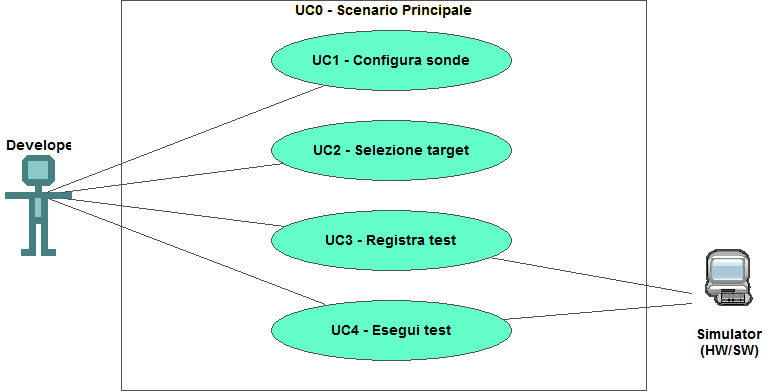
\includegraphics[width=0.9\columnwidth]{usecase/scenario-principale} 
    %\caption{Use Case - UC0: Scenario principale}
%\end{figure}
%
%\begin{usecase}{0}{Scenario principale}
%\usecaseactors{Sviluppatore applicativi}
%\usecasepre{Lo sviluppatore è entrato nel plug-in di simulazione all'interno dell'IDE}
%\usecasedesc{La finestra di simulazione mette a disposizione i comandi per configurare, registrare o eseguire un test}
%\usecasepost{Il sistema è pronto per permettere una nuova interazione}
%\label{uc:scenario-principale}
%\end{usecase}
%
%\section{Tracciamento dei requisiti}
%
%Da un'attenta analisi dei requisiti e degli use case effettuata sul progetto è stata stilata la tabella che traccia i requisiti in rapporto agli use case.\\
%Sono stati individuati diversi tipi di requisiti e si è quindi fatto utilizzo di un codice identificativo per distinguerli.\\
%Il codice dei requisiti è così strutturato R(F/Q/V)(N/D/O) dove:
%\begin{enumerate}
	%\item[R =] requisito
    %\item[F =] funzionale
    %\item[Q =] qualitativo
    %\item[V =] di vincolo
    %\item[N =] obbligatorio (necessario)
    %\item[D =] desiderabile
    %\item[Z =] opzionale
%\end{enumerate}
%Nelle tabelle \ref{tab:requisiti-funzionali}, \ref{tab:requisiti-qualitativi} e \ref{tab:requisiti-vincolo} sono riassunti i requisiti e il loro tracciamento con gli use case delineati in fase di analisi.
%
%\newpage
%
%\begin{table}%
%\caption{Tabella del tracciamento dei requisti funzionali}
%\label{tab:requisiti-funzionali}
%\begin{tabularx}{\textwidth}{lXl}
%\hline\hline
%\textbf{Requisito} & \textbf{Descrizione} & \textbf{Use Case}\\
%\hline
%RFN-1     & L'interfaccia permette di configurare il tipo di sonde del test & UC1 \\
%\hline
%\end{tabularx}
%\end{table}%
%
%\begin{table}%
%\caption{Tabella del tracciamento dei requisiti qualitativi}
%\label{tab:requisiti-qualitativi}
%\begin{tabularx}{\textwidth}{lXl}
%\hline\hline
%\textbf{Requisito} & \textbf{Descrizione} & \textbf{Use Case}\\
%\hline
%RQD-1    & Le prestazioni del simulatore hardware deve garantire la giusta esecuzione dei test e non la generazione di falsi negativi & - \\
%\hline
%\end{tabularx}
%\end{table}%
%
%\begin{table}%
%\caption{Tabella del tracciamento dei requisiti di vincolo}
%\label{tab:requisiti-vincolo}
%\begin{tabularx}{\textwidth}{lXl}
%\hline\hline
%\textbf{Requisito} & \textbf{Descrizione} & \textbf{Use Case}\\
%\hline
%RVO-1    & La libreria per l'esecuzione dei test automatici deve essere riutilizzabile & - \\
%\hline
%\end{tabularx}
%\end{table}%
%**************************************************************
\chapter{Accenni al funzionamento di Alfresco}
\label{cap:architettura}
%**************************************************************

\intro{In questo capitolo viene esposto come creare un modulo e accenni all'architettura di Alfresco}\\

%**************************************************************
\section{Architettura di Alfresco}
Al cuore di Alfresco c'è un repository che fornisce uno spazio per i contenuti, e un ampio spettro di servizi che possono essere utilizzati dalle applicazioni per manipolare il suo contenuto. Il diagramma \ref{fig:architettura-generale} mostra l'idea alla base di Alfresco, che può essere considerato formato da tre principali componenti: la piattaforma (Platform), la User Interface (UI), e la componente di ricerca (Search), basata su Apache Lucene. Queste componenti sono implementate come applicazioni web separate.
\begin{figure}[!ht]
\centering
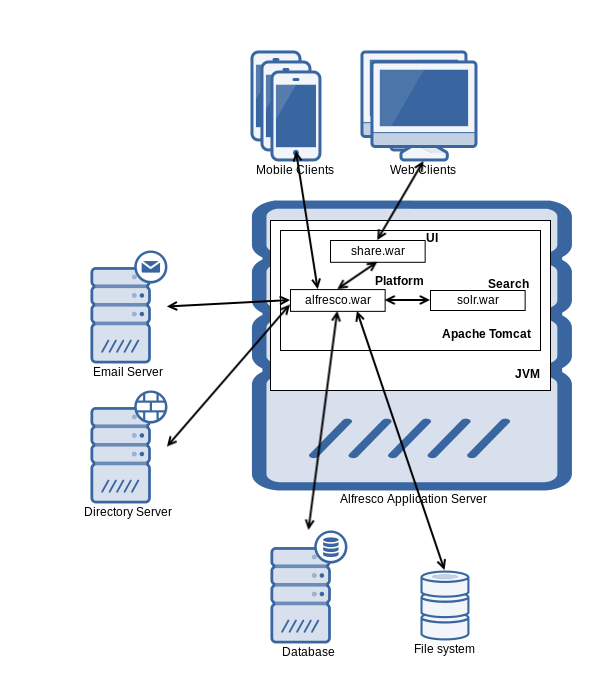
\includegraphics[width=\textwidth]{/architettura/architettura3.png}
\caption{architettura generale}
\label{fig:architettura-generale}
\end{figure}
Il principale componente è chiamato Platform ed è implementato nella web application alfresco.war. Essa fornisce il repository dove i file sono tenuti in memoria oltre a tutti i servizi di accesso e gestione collegati. Alfresco Share fornisce una interfaccia web (UI) per il repository ed è implementata nella web application share.war. Share nasce per facilitare agli utenti la gestione dei loro siti, documenti, utenti e così via.\\
La funzionalità di ricerca è implementata su Apache Solr 4 e fornisce una indicizzazione di tutti i contenuti, che rende possibile una potente funzionalità di ricerca. Oltre ai web client che accedono al repository via Share ci sono anche i dispositivi mobile che possono accedervi tramite le APIs REST fornite dalla piattaforma.

Se si approfondisce il componente Platform (contenuto nell'alfresco.war) vedremo che esso supporta i workflow nella forma dell'integrato Activiti Workflow Engine. La piattaforma di solito, come anche nell'azienda in cui è stato svolto lo stage, viene integrata con un Directory Server (LDAP), per essere in grado di sincronizzare i gruppi e gli utenti con Alfresco Community Edition. La maggior parte delle installazioni, compresa quella di Ennova, integrano Alfresco anche con un server SMTP così il componente Platform può mandare E-mail, come ad esempio, ma non solo, inviti ai siti.

Per maggiori informazioni si rimanda alla visione della documentazione di Alfresco.

Oltre a Share vi sono anche molti altri client che possono connettersi al repository, e questi includono anche molti client compatibili con CMIS, e via il protocollo SharePoint e il client SharePoint. Esiste anche, a pagamento, la possibilità di sincronizzare i contenuti nel cloud.

Platform inoltre contiene numerose APIs, Servizi, e protocolli.

Il diagramma \ref{fig:architettura-estesa} illustra questa architettura estesa

\begin{figure}[!ht]
\centering
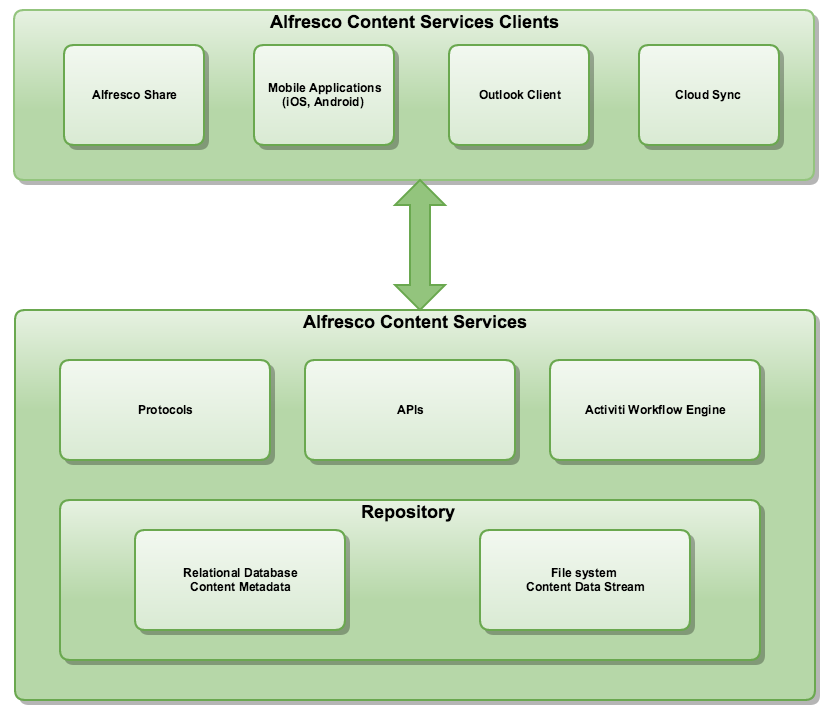
\includegraphics[width=\textwidth]{/architettura/architettura2.png}
\caption{architettura estesa\label{fig:architettura-estesa}}
\end{figure}

Si noti come i metadati del contenuto sono conservati in un database relazionale come PostgreSQL, MySQL, Oracle, e così via. Il contenuto in se è conservato nel file system (o altri sistemi di storage come Amazon S3).

Alfresco fornisce un buon numero di punti di estensione per permettere ad uno sviluppatore di customizzarlo. Questi punti hanno molte forme, tra cui:
\begin{itemize}
\item Platform extension points, illustrati nell'immagine \ref{fig:dev-platform-integration-architecture.png}
\item Share extension points, illustrati nell'immagine \ref{fig:dev-extensions-share-architecture}
\item Platform integration points, illustrati nell'immagine \ref{fig:dev-repo-extension-points.png}
\item APIs
\item Protocolli
\item Servizi
\end{itemize}
\begin{figure}[!ht]
\centering
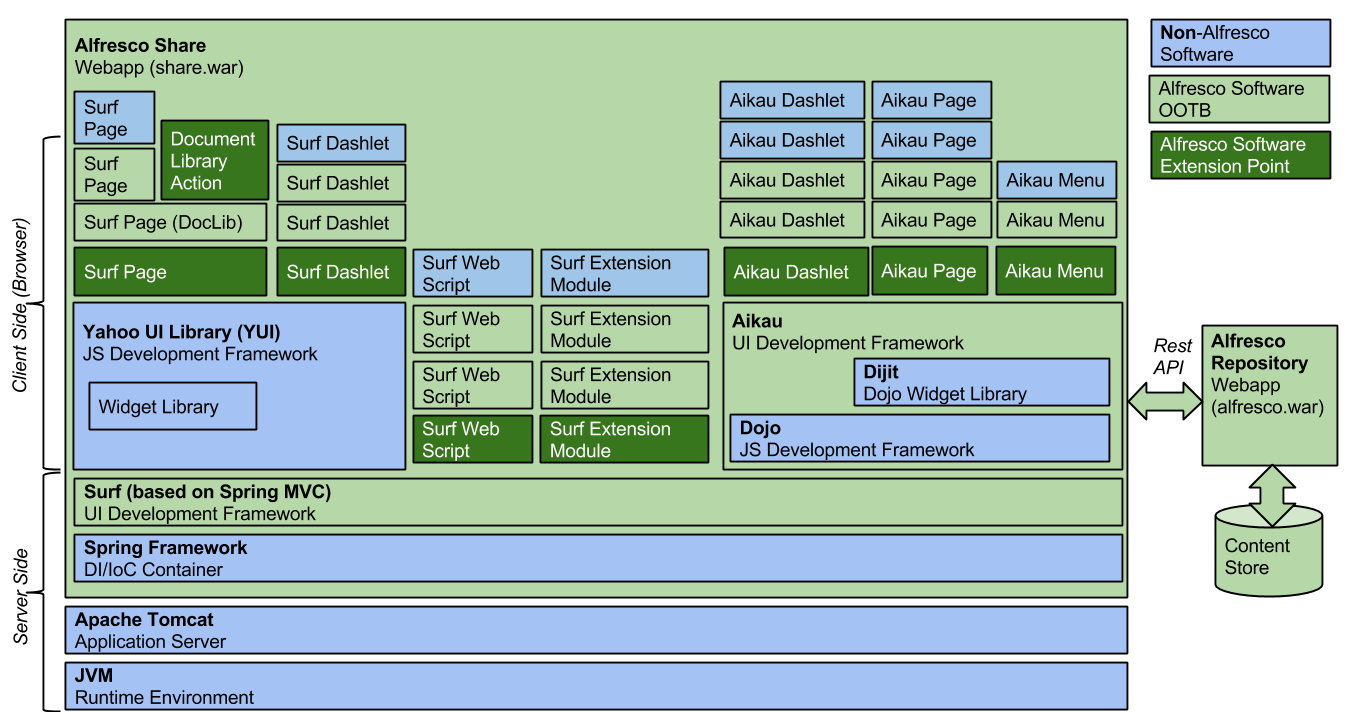
\includegraphics[width=\textwidth]{/architettura/dev-extensions-share-architecture.png}
\caption{Architettura di Share\label{fig:dev-extensions-share-architecture}}
\end{figure}
\begin{figure}[!ht]
\centering
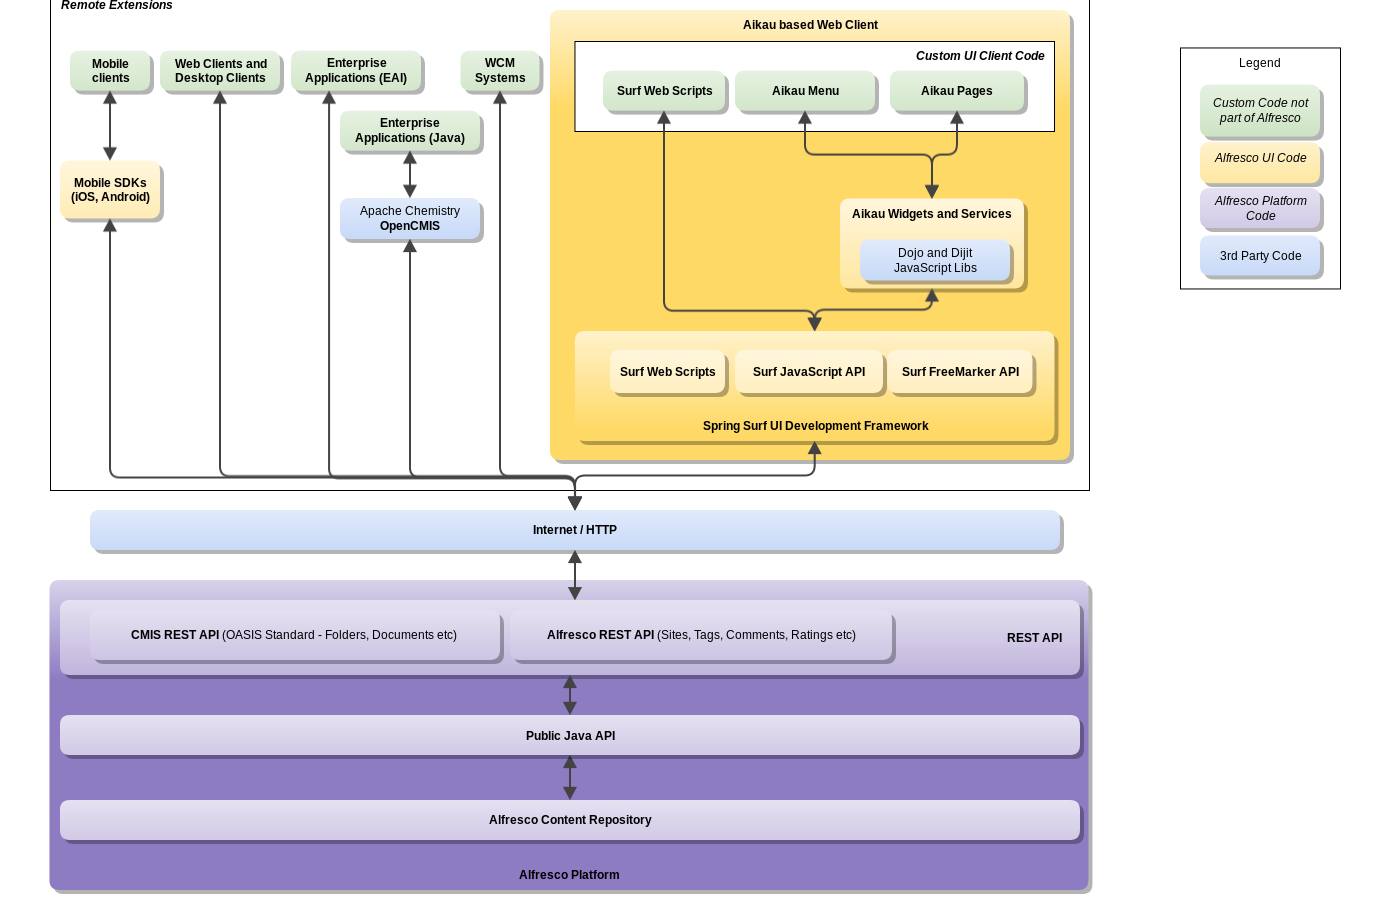
\includegraphics[width=\textwidth]{/architettura/dev-platform-integration-architecture.png}
\caption{Architettura del componente Platform\label{fig:dev-platform-integration-architecture.png}}
\end{figure}
\begin{figure}[!ht]
\centering
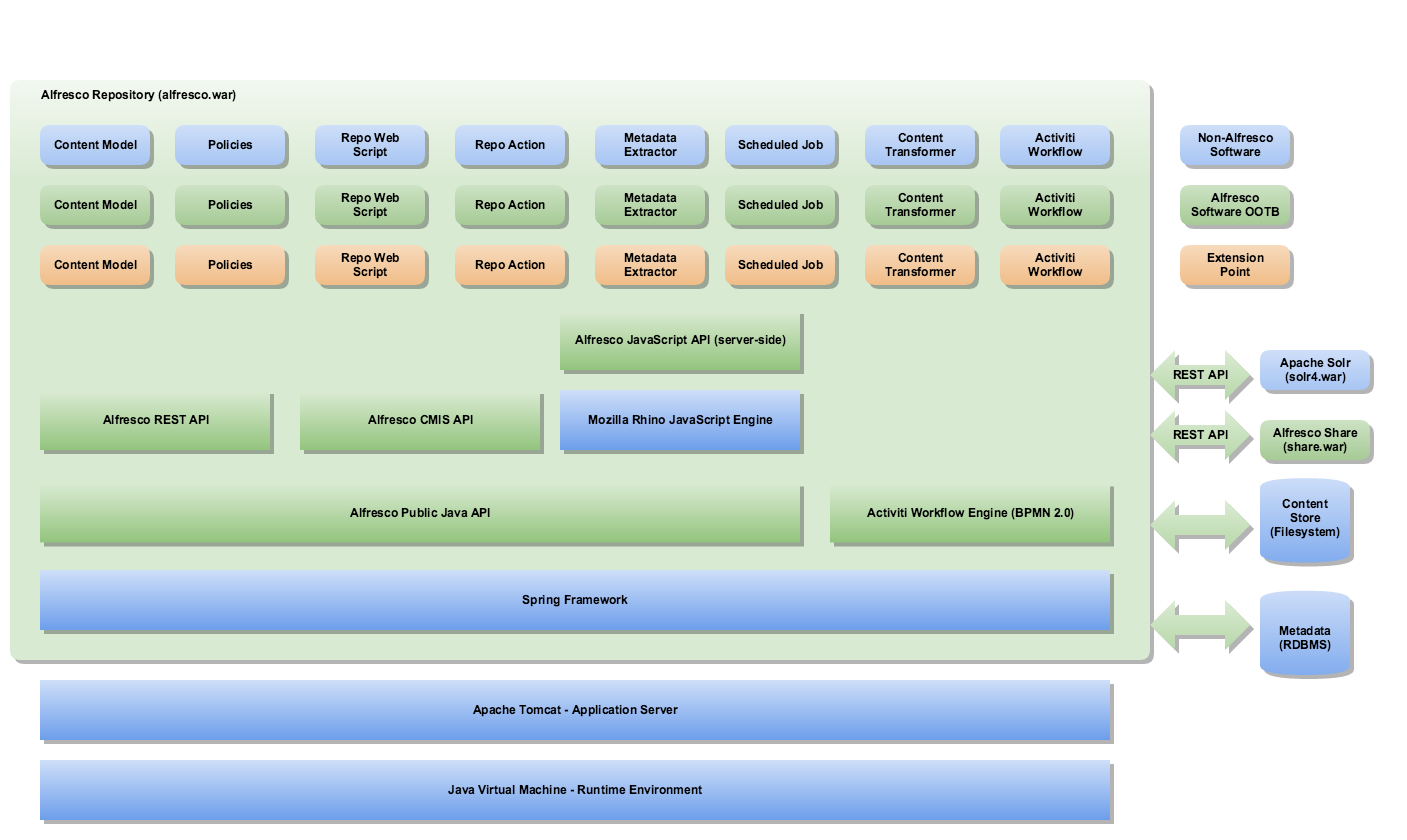
\includegraphics[width=\textwidth]{/architettura/dev-repo-extension-points.png}
\caption{Architettura del Repository\label{fig:dev-repo-extension-points.png}}
\end{figure}
\section{SDK}
L’Alfresco SDK è un kit di sviluppo basato su Maven che fornisce un approccio semplice
da utilizzare per lo sviluppo di applicazioni ed estensioni per Alfresco. Con questa SDK è
possibile sviluppare, testare, eseguire, documentare e rilasciare il proprio modulo od estensione per Alfresco. La SDK fornisce tre archetipi di Maven che possono essere
usati al fine di generare un progetto per Alfresco, e sono pensati per fornire un approccio standardizzato allo sviluppo, rilascio e distribuzione dei prodotti relativi ad Alfresco. È quindi possibile generare i
seguenti tipi di archetipi:
\begin{itemize}
\item Alfresco Repository AMP: questo archetipo si utilizza per creare moduli
per il solo Alfresco Repository Web Application;
\item Alfresco Share AMP: questo archetipo si utilizza per creare moduli per il solo
Alfresco Share Web Application;
\item Alfresco all-in-one (AIO): questo archetipo si utilizza quando vi è necessità di creare un progetto che richieda sia la componente Share che quella Repo, è la più potente e completa delle distribuzioni SDK, ma anche la più pesante.
\end{itemize}
tutti questi archetipi hanno delle caratteristiche comuni, quali:
\begin{itemize}
\item AMP packaging, cioè sono in grado di generare con la loro compilazione i file AMP, che sono i file che contengono i dati che poi verranno installati nei WAR corrispondenti.
\item La gestione delle dipendenze in Maven;
\item La generazione di uno scheletro di base sul quale poter creare il proprio progetto;
\item Il supporto ai test di unità, test che vanno inseriti in un'apposita directory.
\item Facilitazioni per l'integrazione di un progetto negli IDE, come IntelliJ IDEA e Eclipse.
\end{itemize}
\subsection{Repository AMP archetype}
L’Alfresco Repository AMP genera un scheletro di progetto per gestire le estensioni e le
personalizzazioni dell’Alfresco Repository. Questo tipo di archetipo dovrebbe essere utilizzato:
\begin{itemize}
\item  per lo sviluppo di un componente repo che non si vuole distribuire nello stesso modulo di un componente all-in-one, per facilitare il lavoro in progetti di grandi dimensioni, che così possono suddividere il progetto in componenti più piccole.
\item per poter creare un componente che sia riusabile e si possa re-includere a sua volta in componenti all-in-one.
\item per creare un modulo che vada ad interagire con la sola parte repo.
\end{itemize}
Questo archetipo presenta caratteristiche ulteriori:
\begin{itemize}
\item Ha il supporto di un database H2 per simulare il database di Alfresco.
\item supporta test di integrazione e di unità tramite Junit e RAD (rapid application development)
\end{itemize}
\subsection{Share AMP archetype}
Alfresco Share AMP Archetype genera un progetto esempio per gestire le estensioni e
le personalizzazioni di Alfresco Share. Questo tipo di archetipo dovrebbe essere utilizzato per:
\begin{itemize}
\item realizzare un modulo Share per poi includerlo all’interno di un progetto all-in-one;
\item costruire un Add-On, componente, modulo da distribuire separatamente;
\item poter spezzare il lavoro, per esempio per delegare a team diversi il lato front-end e il lato back-end;
\item creare temi e personalizzazioni che coinvolgano il solo lato UI.
\end{itemize}
Anche questo modulo presenta alcune caratteristiche particolari:
\begin{itemize}
\item sono presenti alcuni componenti di esempio per facilitare la creazione di nuove funzionalità
\item può interfacciarsi con qualsiasi componente repo di Alfresco, previa configurazione; questo permette di poter provare in sicurezza tutte le modifiche alla UI apportate direttamente in un ambiente molto vicino a quello di produzione.
\end{itemize}
\subsection{All-in-One archetype}
All-in-One archetype è un progetto multi-modulo per personalizzare ed estendere la
Share e la Repository di Alfresco.Questo tipo di archetipo dovrebbe essere utilizzato per:
\begin{itemize}
\item realizzare un progetto che permetta la personalizzazione in contemporanea e in un singolo modulo della Share e della
Repository;
\item accedere alla suite completa dei test di regressione per la Alfresco Share UI;
\item accedere ai test funzionali basati sulla libreria Alfresco Share Page Object (PO).
\end{itemize}
Le principali caratteristiche di questo archetipo sono:
\begin{itemize}
\item inclusione semplice degli AMPs extra;
\item il supporto ad estensioni Out-of-the-box come la gestione dei records, il protocollo SharePoint, la
gestione dei Media;
\item la possibilità di personalizzare i test funzionali;
\item la replicazione di un'intera distribuzione di Alfresco, che funziona autonomamente e non ha bisogno di dipendenze aggiuntive.
\end{itemize}
Ovviamente questo archetipo è il più pesante, e il suo completo deploy richiede una quantità di tempo non indifferente, per cui andrebbe usato solo se vi è reale necessità di utilizzare tutte le caratteristiche uniche che esso fornisce
\section{Gestione dei moduli}
\subsection{Creazione}
Per poter utilizzare l'SDK è necessario sottostare ai prerequisiti descritti nella pagina dei prerequisiti di installazione di Alfresco\footcite{site:alfresco-prerequisites}.
Fatto questo il progetto può essere importato in un IDE, ad esempio im Eclipse, seguendo le apposite guide nella documentazione di Alfresco\footcite{site:alfresco-rad}
Le cartelle su cui andremo a sviluppare saranno la repo-amp e la share-amp. La share-amp verrà utilizzata per sviluppare l’interfaccia grafica del modulo mentre la parte di repo-amp  per lo sviluppo del “back-end”, le altre folder create servono per replicare l’ambiente di Alfresco in fase di esecuzione del modulo, e quindi non ha senso lavorare su di esse.\\
È necessario installare il driver jdbc se si intende  lavorare nell’SDK interagendo con database terzi, e dato che non è incluso nell'SDK anche se presente nell'ambiente finale, va incluso seguendo quanto descritto nel forum di Alfresco \footcite{site:alfresco-jdbc}. 
Una volta fatto questo, bisogna aprire nell’IDE o anche a mano i vari file di Alfresco, seguendo quanto descritto nelle guide già citate, la cartella contenente la parte che verrà utilizzata per registrare la pagina in Alfresco share, nella cartella contenente le estensioni web e più nello specifico i webscript. %partendo dalla cartella di installazione (sono riportati gli indirizzi utilizzando i nomi dell’esempio sopra citato: %\texttt{/ alfresco-extension / acme-cms-poc / acme-cms-poc-share-amp / src / main / amp / config / alfresco / web-extension / site-webscripts / com / example / pages}
% (questo porta a dove è situata la pagina dimostrativa). È sufficiente fermarsi due o tre livelli sopra se l’intenzione è quella di mettere la gerarchia per una pagina custom (come fatto in questo progetto).
Una pagina fatta in alfresco share è composta da tre file, per semplicità prendiamo in considerazione la pagina di esempio già fornita:
\begin{itemize}
\item un file .xml, che descrive i dati essenziali della pagina, come quello riportato come esempio nel listato \ref{lst:codesempio}
\begin{lstlisting}[language=XML, caption=codice di una pagina di esempio, label=lst:codesempio]
<webscript>
    <shortname>Simple Page</shortname>
    <description>Simple page definition</description>
    <family>Share</family>
    <authentication>user</authentication>
    <url>/simple-page</url>
</webscript>
\end{lstlisting}
molto importanti sono il tag authentication, che specifica il livello di autenticazione necessario per accedere alla pagina, e il tag url, dal momento che definisce l’indirizzo della pagina, che sarà \texttt{<ip>:port/share/page/hdp/ws<url>} (hdp genera la pagina con header e footer, dp la pagina grezza).
\item un file .html che si comporta proprio come il body di una pagina html.
\item un file .js, che serve per applicare delle modifiche via json al model.
\end{itemize}
Quanto detto è sufficiente per creare una pagina che non necessiti di interazioni con Java.

Per quanto riguarda una pagina che invece fa uso delle api di Alfresco il procedimento è più complicato: la pagina che verrà mostrata all’utente è collocata nella cartella contenente i template per i webscripts.
La pagina generata è situata all’indirizzo \texttt{<ip>:<porta>/alfresco/service<url>}.
È inoltre necessario creare un bean che fa da collegamento tra il codice java, situato appunto in una cartella specifica che contiene le classi java, e la pagina che verrà generata. Per farlo seguire quanto descritto nelle guide per la configurazione di Alfresco \footcite{site:alfresco-bean}.

\subsection{Manutenzione}
Nel momento in cui si ha l'intenzione di modificare un modulo per evenienze riguardanti aspetti grafici o logici indiretti, si dovrà aprire il modulo con un IDE a piacere, e applicare le modifiche desiderate sui file.\\
 Il risultato delle modifiche effettuate è visionabile lanciando il comando \texttt{./run.sh} una volta posizionati all’interno della cartella del modulo su linux, \texttt{run.bat} su windows, in alternativa al comando \texttt{mvn install -Prun}  o  \texttt{mvn clean install -Prun}, se è necessario anche svuotare la cache; avviato il server basterà
aprire il browser e digitare l’url : \texttt{<ip>:8080/share/page}.
Per quanto riguarda l’importazione dei moduli nell'ambiente di Alfresco vero e proprio, si dovrà lanciare il comando \texttt{mvn clean install} all'interno sempre del folder del modulo e all’interno della cartella target delle rispettive cartelle repo-amp e share-amp si creeranno un repo-amp file e uno share-amp file. Questi dovranno essere inseriti rispettivamente nelle cartelle amps e amps\_share nell'ambiente dell'Alfresco di produzione.
Per installare il modulo  è necessario lanciare il file \texttt{alfresco-community/bin/apply\_amps.bat}, oppure lanciandolo tramite il flag \texttt{-force} se si ha già un modulo con lo stesso nome che si vuole sovrascrivere.\\
\emph{Attenzione:}L’installazione dei moduli comporta un deploy che sovrascrive il contenuto delle cartelle
\texttt{tomcat/webapps/share} e \texttt{tomcat/webapps/alfresco}. Di conseguenza nel momento in cui si è andati ad effettuare delle estensioni direttamente all’interno di queste cartelle il contenuto andrà perso. Quindi prima di effettuare questa operazione è necessario fare il backup delle cartelle indicate precedentemente.

%\emph{Per comodità d’ora in poi il nome del progetto sarà indicato come AIOProject}.             % Concept Preview
% !TEX encoding = UTF-8
% !TEX TS-program = pdflatex
% !TEX root = ../tesi.tex
% !TEX spellcheck = it-IT
%
%**************************************************************
%/chapter{Progettazione e codifica}
%/label{cap:progettazione-codifica}
%**************************************************************
%
%/intro{Breve introduzione al capitolo}/\
%
%**************************************************************
%/section{Tecnologie e strumenti}
%/label{sec:tecnologie-strumenti}
%
%Di seguito viene data una panoramica delle tecnologie e strumenti utilizzati.
%
%/subsection*{Tecnologia 1}
%Descrizione Tecnologia 1.
%
%/subsection*{Tecnologia 2}
%Descrizione Tecnologia 2
%
%**************************************************************
%/section{Ciclo di vita del software}
%/label{sec:ciclo-vita-software}
%
%**************************************************************
%/section{Progettazione}
%/label{sec:progettazione}
%
%/subsubsection{Namespace 1} %**************************
%Descrizione namespace 1.
%
%/begin{namespacedesc}
    %/classdesc{Classe 1}{Descrizione classe 1}
    %/classdesc{Classe 2}{Descrizione classe 2}
%/end{namespacedesc}
%
%
%**************************************************************
%/section{Design Pattern utilizzati}
%
%**************************************************************
%/section{Codifica}
%**************************************************************
\chapter{Il modulo clienti}
\label{cap:modulo-clienti}
%**************************************************************

\intro{In questo capitolo verrà esposta l'implementazione e le fasi che hanno portato la creazione del modulo clienti}/\

\section{scopo del modulo} il modulo clienti si pone come scopo quello di creare un semplice sistema di CRUD in un database. In questo caso è stato inmplementato in un database Postgres, che è quello che viene incluso con Alfresco Community, ma è stata esplicita richiesta dell'azienda che fosse possibile una configurazione su ambienti simili ma che non fossero esclusivamente Postgres.
\section{implementazione delle funzionalità}
Preparazione del DB
Per preparare il db bisogna innanzitutto creare un nuovo database.

Nel caso del progetto da me sviluppato si è usato PostgreSQL

Basta quindi spostarsi nella cartella di postgresql tramite dos e digitare il comando

createdb -h localhost -p <porta> -U postgres <nome del db>

Bisogna quindi creare una tabella, che verrà chiamata per comodità da adesso clienti.

La tabella ha la seguente struttura 
\begin{lstlisting}
CREATE TABLE clienti
(
  identificativo text NOT NULL,
  name text NOT NULL,
  piva text NOT NULL,
  descr text,
  datainizio text NOT NULL,
  datafine text,
  id bigserial NOT NULL,
  CONSTRAINT clienti\_pkey PRIMARY KEY (id)
  CONSTRAINT clienti\_identificativo\_name\_piva\_descr\_datainizio\_datafine\_key UNIQUE (identificativo, name, piva, descr, datainizio, datafine)
)
\end{lstlisting}
Nel creare la tabella è importante prestare attenzione al fatto che l'owner della tabella debba essere il medesimo che è stato settato nelle properies.
L’ultimo vincolo è necessario per non avere record che differiscano solo per id.
In particolare si è scelto di tenere le date in formato testuale per rendere il db compatibile a diverse implementazioni sulla rappresentazione della data, e si è scelto di usare come chiave primaria un id chiamato bigserial, in quanto più resistente ad una eventuale estensione dei campi della tabella e più comodo da utilizzare, dal momento che, per le caratteristiche del bigserial, si è certi che l’ultima versione di un record è quella con l’id più alto, quindi per prendere l’ultima versione di un cliente di un derterminato  identificativo basta eseguire la query \texttt{select * from clienti where id = (select max(id) from clienti where identificativo='param1')}. Si è cercato di non utilizzare viste o altri strumenti particolari per evitare di essere troppo dipendenti dalla piattaforma.



\subsection{Creazione della parte share}

È quindi stato necessario creare le pagine share e le pagine repo, oltre ai bean di collegamento per poter rendere accessibile il webscript. Si è adottato il metodo POST in tutti quante le invocazioni, in quanto è più sicuro e permette lo scambio di una maggiore quantità di dati.

SI è aggiunta innanzitutto una nuova voce di menu aggiungendo il file \texttt{/ AIOProject-share-amp / src / main / amp / config / alfresco / web-extension / site-data / extensions / add-create-menuitem-doclib-extension-modules.xml}
\begin{lstlisting}[language=XML]
<extension>
    <modules>
        <!-- This module is dependent on the custom content model setup in the repo-amp module -->
        <module>
            <id>Add a new menu item to Create... menu in DocLib</id>
            <version>1.0</version>
            <auto-deploy>true</auto-deploy>
            <configurations>
                <config evaluator="string-compare" condition="DocumentLibrary">
                    <create-content>
                        <content id="text-label-clienti" label="Crea nuovo cliente" icon="text" type="pagelink">
                            <param name="page">hdp/ws/clienti</param>
                        </content>
                    </create-content>
                </config>
                            </configurations>
        </module>
    </modules>
</extension>
\end{lstlisting}

Per ulteriore documentazione si faccia riferimento a al \href{http://docs.alfresco.com/5.0/tasks/dev-extensions-share-tutorials-add-menuitem-create-menu.html}{relativo capitolo nella documentazione di alfresco}

Le pagine includono inoltre nell’HTML la richiesta di JQuery, mediante le linee
\begin{lstlisting}
<script src="https://ajax.googleapis.com/ajax/libs/jquery/1.12.4/jquery.min.js"></script>
<link rel="stylesheet" href="https://maxcdn.bootstrapcdn.com/bootstrap/3.3.7/css/bootstrap.min.css" integrity="sha384-BVYiiSIFeK1dGmJRAkycuHAHRg32OmUcww7on3RYdg4Va+PmSTsz/K68vbdEjh4u" crossorigin="anonymous">
\end{lstlisting}

\subsubsection{pagina Clienti}

È la pagina di inserimento di un nuovo cliente ed è composta da un semplice form.
È composta dai seguenti file:
\begin{itemize}
\item \texttt{/ AIOProject-share-amp / src / main / amp / config / alfresco / web-extension / site-webscripts / com / clienti / pages / clienti.get.desc.xml}, implementato come descritto nel \hyperref[cap:architettura]{ quarto  capitolo}
\item\texttt{/ AIOProject-share-amp / src / main / amp / config / alfresco / web-extension / site-webscripts / com / clienti / pages / clienti.get.html.ftl }che contiene il codice html necessario a generare il form.
\item\texttt{/ AIOProject-share-amp / src / main / amp / config / alfresco / web-extension / site-webscripts / com / clienti/ pages / clienti.get.js} che contiene le istruzioni necessarie a generare l’header. È necessario includere nell’html la linea <@processJsonModel group="share"/>.
\item \texttt{/AIOProject-share-amp/src/main/amp/web/js/clienti/clienti.js,} incluso con la linea \texttt{<script src="\${url.context} / js / clienti / clienti.js"></script>}, che effettua i controlli javascript della pagina. In particolare alla pressione del pulsante di conferma viene fatto il controllo sui dati inseriti, cioè sulla correttezza della partita iva, sul fatto che i campi obbligatori siano definiti, sul fatto che la data di fine sia successiva alla data di inizio. Inoltre si occupa di inoltrare la richiesta AJAX al webscript \texttt{query\_processor.java} che sarà trattato successivamente. Se il webscript riporta uno stato anomalo viene segnalato e così viene anche gestito il caso di inserimento di un identificativo già esistente.
\end{itemize}

\subsubsection{Pagina vis\_clienti}

La pagina vis\_clienti è la pagina di gestione dei clienti, ed è suddivisa nei file:
\begin{itemize}
\item \texttt{/ AIOProject-share-amp / src / main / amp / config / alfresco / web-extension / site-webscripts / com / visualizza\_clienti / pages / vis\_clienti.get.desc.xml} che funziona come descritto nel \hyperref[cap:architettura]{ quarto  capitolo}.
\item \texttt{/ AIOProject-share-amp / src / main / amp / config / alfresco / web-extension / site-webscripts / com / visualizza\_clienti / pages / vis\_clienti.get.html.ftl} che fornisce lo scheletro della pagina, che verrà poi popolata tramite richieste AJAX delle parti dinamiche.
\item \texttt{/ AIOProject-share-amp / src / main / amp / config / alfresco / web-extension / site-webscripts / com  /visualizza\_clienti / pages / vis\_clienti.get.js}, che funziona come descritto prima.
\item \texttt{/ AIOProject-share-amp / src / main / amp / web / css / vis\_clienti / vis\_clienti.css}, incluso in maniera analoga al javascript come descritto prima e che definisce il CSS della pagina.
\item \texttt{/ AIOProject-share-amp / src / main / amp / web / js / vis\_clienti / vis\_clienti.js}, incluso come descritto prima
\end{itemize}
In particolare la pagina nella sua parte principale offre la lista degli identificativi dei clienti attivi e non, che è anche il nome con cui sono stati salvati nella cartellatura di Alfresco. Si è scelto questa rappresentazione in quanto è logicamente vicina alla struttura di Alfresco e sarà più facile in futuro implementare funzionalità quali la visualizzazione dei progetti del cliente.  I pulsanti dei clienti attivi e inattivi sono generati rispettivamente da \texttt{clients.java}  e  \texttt{inactive.java}  chiamati all’avvio della pagina tramite \texttt{window.onload} che si occupano di definire anche i giusti parametri che verranno poi utilizzati per popolare il form che consente l’aggiornamento dei dati di un particolare cliente. Il form è già presente nella pagina ma viene fatto mostrare da una opportuna funzione javascript che si occupa anche di popolare la tabella sottostante tramite una chiamata AJAX al webscript \texttt{TablePageGenerator.java}, che si occupa di fornire la tabella e di iniettare il pulsante cancella e il pulsante  per definire  la data di fine del rapporto  con il corretto id. I pulsanti sono collegati a loro volta a \texttt{delete.java} e \texttt{update.java}, chiamati tramite opportune chiamate AJAX.

I messaggi di errore e di conferma sono gestiti dove possibile in JavaScript e dove non possibile, poiché la risposta dipende dal database o dal repository, tramite la risposta della chiamata AJAX

Per riassumere la pagina fa uso delle seguenti funzioni JavaScript:
\begin{itemize}
\item \texttt{set\_table(identificativo)} che si occupa di generare la tabella di un determinato cliente tramite richiesta AJAX
\item \texttt{detail(id,nome,pi,descr,datainizio,datafine)}che si occupa di settare 
E mostrare il dettaglio di un cliente
\item \texttt{controllaPIVA(pi)} che esegue semplicemente  il controllo della partita IVA
\item \texttt{sendRequest()} Che invia la richiesta AJAX di aggiornamento di un determinato cliente
\item \texttt{set\_data\_fine(ID)} che setta la data di fine di un determinato record di un cliente tramite richiesta AJAX
\item \texttt{cancella(key)} che fa la richiesta tramite AJAX di cancellazione di un record con un determinato ID
\item \texttt{up()} che popola la pagina con i pulsanti dei clienti, tramite richiesta AJAX.
\item \texttt{vai(name)} che reindirizza alla cartella con dato nome.
\end{itemize}
Sono presenti altre funzioni che svolgono compiti banali quale la codifica e decodifica di entità, per garantire il funzionamento della pagina nel caso i record contengano caratteri speciali



\subsection{Creazione della parte repo}
\subsubsection{Creazione delle variabili del modulo}
Per rendere possibile la modifica di alcune configurazioni anche dopo che il modulo è stato installato in alfresco, si è provveduto a creare un file in \texttt{/ AIOProject-repo-amp / src / main / amp / config / alfresco / module / AIOProject-repo-amp / config / configModule.properties}, Accessibile da java aggiungendo al codice le linee:
\begin{lstlisting}[language=Java]
private static Properties properties=new Properties();

public static final String getValue(String value) {
		return properties.getProperty(value);
	}
	
properties.load(getClass().getResourceAsStream("/alfresco/module/AIOProject-repo-amp/config/configModule.properties"));
\end{lstlisting}
Questo permette quindi di recuperare le variabili, che si è cercato di documentare direttamente sul codice tramite nomi significativi e una breve descrizione:
\begin{lstlisting}
#query configuration
queryselection=select id,name, piva, datainizio, datafine, descr from clienti where identificativo='param1' order by id
querylastversion=select * from clienti where id = (select max(id) from clienti where identificativo='param1')
queryselectactive=select distinct identificativo from clienti where NOT (datafine IS NOT NULL)
queryselectnotactive=select distinct identificativo from clienti where datafine IS NOT NULL and identificativo not in (select distinct identificativo from clienti where NOT (datafine IS NOT NULL))
#do not use values in the form paramX! They may be sobstituted!
queryselectionwithclause=select param1 from param2 where param3
queryinsertion=insert into param1 values ('param2','param3','param4', 'param5', 'param6', 'param7')
queryupdate=UPDATE param1 SET param2 = 'param3' WHERE id = 'param4';
querydelete=DELETE FROM param1 WHERE id = 'param2';
#set param1 in the previous query
querytable=Clienti
#server configuration
serverip=127.0.0.1
serverid=alfresco
serverpassword=admin
serverport=5432
servername=<nome del database creato>
servertype=postgresql
serverconnector=jdbc
#path in lucene, in the form of PATH:/"/{directory}, the "/"" character is needed 
#because without it it will be escaped by java, java alone puts the final " so 
#you must not put it when you write the query
installationpath=PATH:/"/app:company\_home/st:sites/cm:er/cm:documentLibrary/cm:\_x0030\_2\_x0020\_-\_x0020\_Clients
#down here you can put the names for the folder that are in the client subdirectory
folder.one=01 - Projects
folder.two=02 - General Contracts
folder.three=tre
folder.four=quattro
folder.five=cinque
\end{lstlisting}
Come si vede dove necessario si è cercato di parametrizzare le funzioni.


\subsubsection{Creazione dei webscript}
Come già accennato, le pagine in share per il loro completo funzionamento necessitano di webscript di supporto, per interrogare il database e generare le tabelle contenenti i dati.  Tutti quanti estendono la classe AbstractWebScript, sono contattabili tramite POST e fanno uso del JDBC per contattare il server remoto dove è presente la tabella. Il file .properties descritto prima permette di cambiare secondo le necessità la configurazione della connessione, definita nella riga
\begin{lstlisting}
connection=DriverManager.getConnection((connector+":"+type+"://"+ip+":"+port+"/"+server),id,password);
\end{lstlisting}
Che sono i parametri definiti nel paragrafo query configuration del .properties

I WebScript sono poi registrati nel file \texttt{/ AIOProject-repo-amp / src / main / amp / config / alfresco / module / AIOProject-repo-amp / context / webscript-context.xml} secondo le modalità già descritte.

Per comodità nella chiamata l’indirizzo è stato settato con lo stesso nome della funzione java ad esso corrispondente. Inoltre alcuni  accettano parametri in JSON definiti in coppie \texttt{{key:value}} in un JSonObject

Passiamo ora in rassegna i vari webscript implementati, in ordine alfabetico.
\paragraph{clients.java}
Questo webscript, situato in \texttt{/ AIOProject-repo-amp / src / main / java / clients.java} e dalla pagina definita in \texttt{/ AIOProject-repo-amp / src / main / amp / config / alfresco / extension / templates / webscripts / clients.post.desc.xml} e in \texttt{/ AIOProject-repo-amp / src / main / amp / config / alfresco / extension / templates / webscripts / clients.post.html.ftl}, si occupa di generare i pulsanti necessari a visualizzare poi la pagina di dettaglio per un utente attivo. Si occupa quindi di interrogare il database e di definire di conseguenza i parametri dei pulsanti e il loro nome, che chiamano uno la funzione \texttt{detail(id,nome,pi,descr,datainizio,datafine)},e l’altro la funzione \texttt{vai(name)}. Si appoggia sulla query definita in queryselectactive per selezionare gli utenti attivi, percorrendo poi il result set per di volta in volta assegnare i parametri.
Viene chiamato senza parametri.
La classe si compone delle seguenti funzioni:
\begin{itemize}
\item \texttt{getValue(String value)}, che recupera una property con una data value.
\item \texttt{inizialize\_values ()}, che inizializza le variabili utilizzate, recuperandole dalle properties.
\item \texttt{public void execute(WebScriptRequest req, WebScriptResponse res)} metodo obbligatorio che si può intendere come il metodo che viene invocato alla chiamata Ajax del webscript e che contiene le istruzioni per gestirla.
\item \texttt{execute(Connection con, String query, WebScriptResponse res)}, metodo che esegue la query.
\item \texttt{writedata(ResultSet rs, String result, Connection con)}, metodo che si occupa di ritornare il codice html necessario a generare i pulsanti dei clienti attivi
\end{itemize}
\paragraph{delete.java}
Questo webscript, situato in \texttt{/ AIOProject-repo-amp / src / main / java / delete.java} e dalla pagina definita in \texttt{/ AIOProject-repo-amp / src / main / amp / config / alfresco / extension / templates / webscripts / delete.post.desc.xml} e in \texttt{/ AIOProject-repo-amp / src / main / amp / config / alfresco / extension / templates / webscripts  /delete.post.html.ftl}  si occupa semplicemente di cancellare un elemento che abbia un determinato id, fornito come parametro della chiamata. Si appoggia sulla query definita alla voce querydelete.
La classe si compone delle seguenti funzioni:
\begin{itemize}
\item \texttt{getValue(String value)}, che recupera una property con una data value
\item \texttt{inizialize\_values ()}, che inizializza le variabili utilizzate, recuperandole dalle properties.
\item \texttt{public void execute(WebScriptRequest req, WebScriptResponse res)} metodo obbligatorio che si può intendere come il metodo che viene invocato alla chiamata Ajax del webscript e che contiene le istruzioni per gestirla.
\item \texttt{execute(Connection con, String query)}, metodo che esegue la query di delete di un dato record del database.
\end{itemize}
\paragraph{inactive.java}
Questo webscript, situato in \texttt{/ AIOProject-repo-amp/src/main/java/inactive.java} e dalla pagina definita in \texttt{/ AIOProject-repo-amp / src / main / amp / config / alfresco / extension / templates / webscripts / inactive.post.desc.xml} e in \texttt{/ AIOProject-repo-amp / src / main / amp / config / alfresco / extension / templates / webscripts / inactive.post.html.ftl} si occupa di generare i pulsanti necessari a visualizzare poi la pagina di dettaglio per un utente non più attivo. Si occupa quindi di interrogare il database e di definire di conseguenza i parametri del pulsante e il suo nome, che chiama la funzione \texttt{detail(id,nome,pi,descr,datainizio,datafine)}. Si appoggia sulla query definita in queryselectnotactive per selezionare gli utenti non attivi. Percorrendo poi il result set per di volta in volta assegnare i parametri.
Viene chiamato senza parametri.
La classe si compone delle seguenti funzioni:
\begin{itemize}
\item \texttt{getValue(String value)}, che recupera una property con una data value
\item \texttt{inizialize\_values ()}, che inizializza le variabili utilizzate, recuperandole dalle properties.
\item \texttt{public void execute(WebScriptRequest req, WebScriptResponse res)} metodo obbligatorio che si può intendere come il metodo che viene invocato alla chiamata Ajax del webscript e che contiene le istruzioni per gestirla.
\item \texttt{execute(Connection con, String query, WebScriptResponse res)}, metodo che esegue la query.
\item \texttt{writedata(ResultSet rs, String result, Connection con)}, metodo che si occupa di ritornare il codice html necessario a generare i pulsanti dei clienti non attivi.
\end{itemize}
Si è deciso di renderla autonoma rispetto a clients per consentire una migliore estensione ad ulteriori eventuali funzionalità.
\paragraph{query\_processor.java}
Questo webscript, situato in \texttt{/ AIOProject-repo-amp / src / main / java / query\_processor.java} e dalla pagina definita in \texttt{/ AIOProject-repo-amp / src / main / amp / config / alfresco / extension / templates / webscripts / query\_processor.post.desc.xml} e in \texttt{/ AIOProject-repo-amp / src / main / amp / config / alfresco / extension / templates / webscripts / query\_processor.post.html.ftl} . Si occupa di inserire un oggetto nel database, utilizzando la query definita in  queryinsertion e deve essere chiamato con i seguenti parametri:
\begin{itemize}
\item ID:l’identificativo del cliente,
\item Nome:il nome esteso del cliente,
\item Piva:la partita iva del cliente,
\item Descr:una descrizione generica,
\item Datainizio:la data di inizio del rapporto,
\item Datafine:la data di fine del rapporto(se non presente, verrà settata a null),
\item Mode:1=inserimento con la creazione delle cartelle, 2=inserimento senza creazione di cartelle ,
\item Box1:creazione della cartella di nome definito in folder.one ,
\item box2:creazione della cartella di nome definito in folder.two ,
\item box3:creazione della cartella di nome definito in folder.three ,
\item box4:creazione della cartella di nome definito in folder.four ,
\item box5:creazione della cartella di nome definito in folder.five ,
\end{itemize}
Lo script si appoggia, oltre al JDBC per l’inserimento nel database, sulla API di Alfresco 
FileFolderService per creare la gerarchia di cartelle corrispondente, di permissionservice per settare i permessi di accesso alle cartelle (per il momento codificati nel Java e non configurabili dopo l’installazione se non mediante l’editor dei permessi di Alfresco)
E di nodeservice per settare la descrizione della cartella principale.
Per includere il serviceregisty, necessario per accedere alla API di Alfresco, è necessario, oltre a specificare  nel bean, il cui funzionamento è stato già descritto, tramite le righe
\begin{lstlisting}[language=XML]
        <property name="serviceRegistry">
          <ref bean="ServiceRegistry" />
      </property>
\end{lstlisting}
E poi nel codice java con l’aggiunta di
\begin{lstlisting}[language=Java]
import org.alfresco.service.ServiceRegistry;

private ServiceRegistry serviceRegistry;

public void setServiceRegistry(ServiceRegistry serviceRegistry) {
		this.serviceRegistry = serviceRegistry;
	}
\end{lstlisting}
Ritorna una stringa di risultato dove è specificato l’esito dell’operazione.
La classe si compone delle seguenti funzioni:
\begin{itemize}
\item \texttt{setServiceRegistry(ServiceRegistry serviceRegistry)}, che inizializza il parametro per il service registry di Alfresco. È richiesto obbligatoriamente da Alfresco se si vogliono utilizzare le sue funzionalità
\item \texttt{getValue(String value)}, che recupera una property con una data value
\item \texttt{inizialize\_values ()}, che inizializza le variabili utilizzate, recuperandole dalle properties.
\item \texttt{public void execute(WebScriptRequest req, WebScriptResponse res)} metodo obbligatorio che si può intendere come il metodo che viene invocato alla chiamata Ajax del webscript e che contiene le istruzioni per gestirla.
\item \texttt{execute(Connection con, String query)}, metodo che esegue la query.
\item \texttt{create\_folder\_tree(String ID, String descr,Boolean box1, Boolean box2, Boolean box3, Boolean box4, Boolean box5)}, metodo che si occupa di creare la cartellatura di un nuovo cliente, di settare i permessi alle cartelle e di settare la descrizione della cartella padre.
\end{itemize}
\paragraph{TablePageGenerator.java}
Questo webscript, situato in \texttt{/ AIOProject-repo-amp / src / main / java / TablePageGenerator.java} e dalla pagina definita in \texttt{/AIOProject-repo-amp / src / main / amp / config / alfresco / extension / templates / webscripts / TablePageGenerator.post.desc.xml} e in \texttt{/ AIOProject-repo-amp / src / main / amp / config / alfresco / extension / templates / webscripts / TablePageGenerator.post.html.ftl}  si occupa di generare la tabella dello storico di un determinato codice cliente, fornito come parametro della chiamata AJAX. Si appoggia sulla query definita alla voce queryselection.
Il webscript si occupa di generare il codice della tabella e di iniettare i giusti parametri nel pulsante per cancellare, e, nel caso la data di fine non sia stata settata, anche di generare il pulsante per la modifica della data di fine rapporto.
La classe si compone delle seguenti funzioni:
\begin{itemize}
\item \texttt{getValue(String value)}, che recupera una property con una data value
\item \texttt{inizialize\_values ()}, che inizializza le variabili utilizzate, recuperandole dalle properties.
\item \texttt{public void execute(WebScriptRequest req, WebScriptResponse res)} metodo obbligatorio che si può intendere come il metodo che viene invocato alla chiamata Ajax del webscript e che contiene le istruzioni per gestirla.
\item \texttt{execute(Connection con, String query, WebScriptResponse res)}, metodo che esegue la query.
\item \texttt{dumpData(ResultSet rs, String result)}, metodo che si occupa di ritornare il codice html necessario a generare la tabella dello storico di un cliente.
\end{itemize}
\paragraph{update.java}
Questo webscript, situato in \texttt{/ AIOProject-repo-amp / src / main / java / update.java} e dalla pagina definita in \texttt{/ AIOProject-repo-amp / src / main / amp / config / alfresco / extension / templates / webscripts / update.post.desc.xml} e in \texttt{/ AIOProject-repo-amp / src / main /amp / config / alfresco / extension / templates / webscripts / update.post.html.ftl}  si occupa semplicemente di cancellare un elemento che abbia un determinato id, un campo da aggiornare e un valore con cui aggiornarlo,  forniti come parametro della chiamata. Si appoggia sulla query definita alla voce queryupdate.
La classe si compone delle seguenti funzioni:
\begin{itemize}
\item \texttt{getValue(String value)}, che recupera una property con una data value
\item \texttt{inizialize\_values ()}, che inizializza le variabili utilizzate, recuperandole dalle properties.
\item \texttt{public void execute(WebScriptRequest req, WebScriptResponse res)} metodo obbligatorio che si può intendere come il metodo che viene invocato alla chiamata Ajax del webscript e che contiene le istruzioni per gestirla.
\item \texttt{executeupdate(Connection con, String query)}, metodo che esegue la query di update della data di fine di un dato record del database.
\end{itemize}

\section{lato estetico}
Per il lato estetico si è reso necessario contattare il team di grafici che lavora presso l'azienda per ottenere un aspetto gradevole e che si allineasse con quanto già presente in Alfresco. Sono stati quindi forniti dei mockup delle varie componenti ed è stato chiesto allo stagista di riprodurre tale aspetto in Alfresco.
\subsection{risultati raggiunti}
TODO:qui le immagini             % Product Prototype
% !TEX encoding = UTF-8
% !TEX TS-program = pdflatex
% !TEX root = ../tesi.tex
% !TEX spellcheck = it-IT

%**************************************************************
%\chapter{Verifica e validazione}
%\label{cap:verifica-validazione}
%**************************************************************
\chapter{Il modulo progetti}
\label{cap:modulo-progetti}
%**************************************************************

\intro{In questo capitolo verrà esposta l'implementazione e le fasi che hanno portato la creazione del modulo progetti}\\

\section{Scopo del modulo} Il modulo progetti, come quello clienti, si pone come scopo quello di creare un semplice sistema di CRUD in un database. Anche in questo caso valgono le considerazioni fatte riguardo al DB e in più è stata richiesta la possibilità di inviare mail a coloro i quali è stato assegnato il progetto e la assegnazione intelligente dei permessi di visualizzazione delle cartelle create a coloro i quali è stato assegnato un progetto.\\

Questo modulo si basa fortemente sulle tecniche e le funzioni già implementate e descritte durante l'esposizione del precedente modulo, tuttavia si è cercato di eseguire la  maggior parte del lavoro di composizione delle pagine tramite JavaScript, per testare la velocità di questa soluzione rispetto a quella adottata prima sia in termini di prestazioni che di tempi di sviluppo. Inoltre è stata inserita una integrazione con LDAP.

Il progetto punta a sfruttare il modulo di inserimento dei clienti per aggiungere nuove funzionalità.
A tale scopo, anche il modulo riguardante i clienti andrebbe aggiornato, per sfruttare tutte le funzionalità introdotte. Tuttavia il modulo clienti è completamente funzionante anche stand alone, mentre il modulo di un nuovo progetto è pensato per funzionare in abbinamento con il modulo della gestione dei clienti e necessita di esso.
\section{Presentazione generale del modulo}
Nella figura \ref{fig:cartelle-progetti} si illustra in generale quanto è stato prodotto per questo modulo. In seguito, nella descrizione di dettaglio, si indicheranno i nomi specifici dei file più importanti che sono stati creati
\begin{figure}[!ht]
\centering
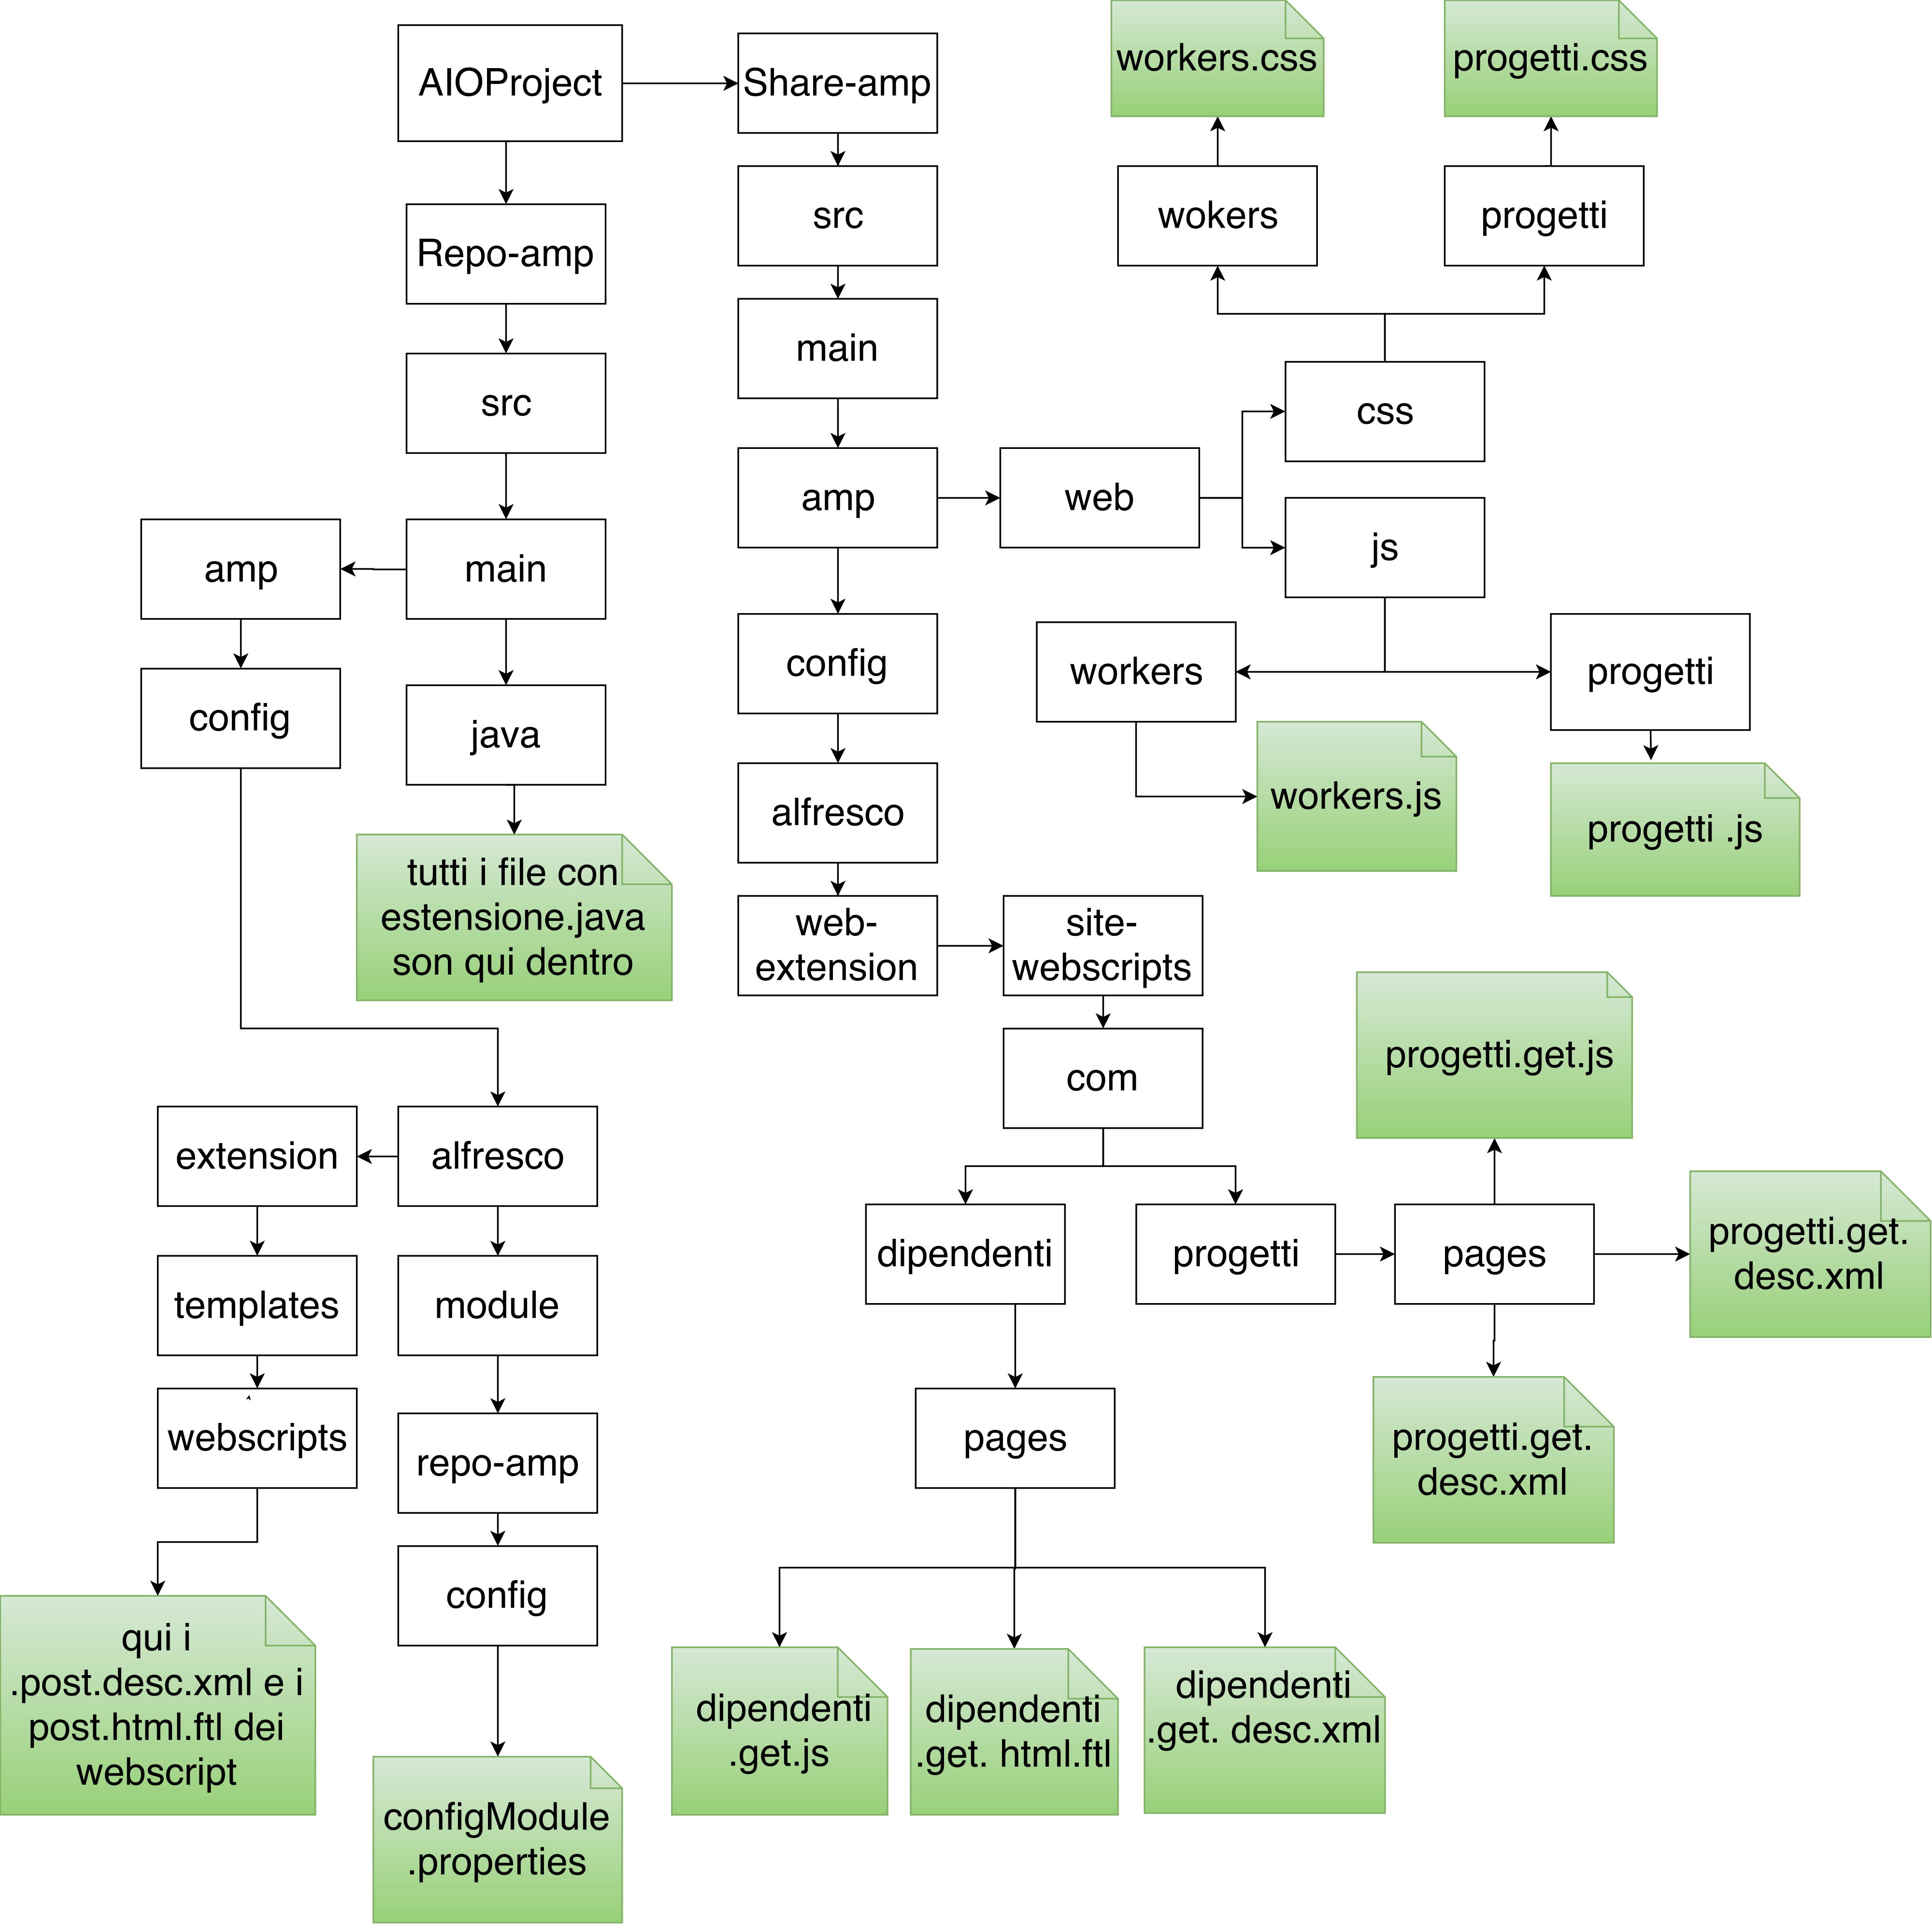
\includegraphics[width=\textwidth]{/diagrammi_cartelle/progettifolder.png}
\caption{descrizione generale di quanto creato per il modulo relativo ai progetti\label{fig:cartelle-progetti}}
\end{figure}
\section{Implementazione delle funzionalità}
\subsection{Aggiunte al DB}
Per il corretto funzionamento del modulo è stato necessario aggiungere le tabelle, il cui codice necessario per la loro generazione è riportato nei listati \ref{lst:table-progetti} e \ref{lst:table-lavoratori}
\begin{lstlisting}[language=SQL,caption=codice per la tabella progetti, label=lst:table-progetti]
CREATE TABLE progetti
(
  nome text NOT NULL,
  descr text,
  CONSTRAINT progetti_pkey PRIMARY KEY (nome)
)
\end{lstlisting}
La tabella relativa ai progetti, riportata nel listato \ref{lst:table-progetti} è una tabella che semplicemente deve contenere la lista dei progetti e la loro descrizione (si assume  che il nome di un progetto sia univoco, altrimenti basterebbe aggiungere un id in auto\_increment alla tabella). La seguente tabella è stata pensata per garantire la possibilità di aggiunta di attributi ad un progetto,  senza aggiungere complessità alla tabella di coloro che sono impiegati in un progetto.
È necessaria per poter gestire il caso di un progetto senza alcun assegnatario, ed in futuro verrà sicuramente espansa all'aggiunta di nuove funzionalità.

Più degna di nota è la tabella delle persone impegnate su un progetto, riportata nel listato \ref{lst:table-lavoratori}

\begin{lstlisting}[language=SQL,caption=codice per la tabella lavoratori, label=lst:table-lavoratori]
CREATE TABLE lavoratori
(
  mail text NOT NULL,
  project text NOT NULL,
  client serial NOT NULL,
  descr text,
  CONSTRAINT lavoratori_pkey PRIMARY KEY (mail, project, client),
  CONSTRAINT lavoratori_client_fkey FOREIGN KEY (client)
      REFERENCES clienti (id) MATCH SIMPLE
      ON UPDATE NO ACTION ON DELETE NO ACTION
)
\end{lstlisting}

Come si vede vi è qui diretto collegamento tra il progetto e il cliente che lo ha commissionato (si assume nell’assegnazione del progetto che la versione del cliente a cui viene assegnato un progetto sia quella dell’ultima modifica nota eseguita tramite il modulo clienti. Ciò è garantito del fatto di selezionare l’id maggiore, in quanto il tipo serial dell’id cliente non decresce alla cancellazione di un record; si ha quindi la certezza che ad un dato nome di un cliente, la sua ultima versione è quella con id maggiore.

\subsection{Definizione delle properties}

Il sistema fa uso delle seguenti properties, riportate nel listato \ref{lst:properties-progetti} per far capire meglio le query utilizzate.
\begin{lstlisting}[label=lst:properties-progetti,caption=properties del modulo relativo ai progetti]
#query configuration
queryselectallprojects=select project,mail,lavoratori.descr,identificativo from lavoratori join clienti on Client=ID order by project
queryselectallclients=select distinct identificativo from clienti
#do not use values in the form paramX! They may be sobstituted!
insertworker=insert into lavoratori values ('value1','value2',(select max(ID) from clienti where identificativo='value3'),'value4');
insertproject= insert into progetti values ('value2','value4')
#server configuration
serverip=localhost
serverid=alfresco
serverpassword=admin
serverport=5432
servername=testdb
servertype=postgresql
serverconnector=jdbc
ldap.authentication.java.naming.provider.url=ldap://192.168.55.73:389
#path in lucene, in the form of PATH:\"/{directory}, the "\"" character is needed 
#because without it it will be escaped by java, java alone puts the final " so 
#you must not put it when you write the query
clientinstallationpath=PATH:\"/app:company_home/st:sites/cm:er/cm:documentLibrary/cm:_x0030_2_x0020_-_x0020_Clients/cm:put_name_here/cm:_x0030_1_x0020_-_x0020_Projects
#down here you can put the names for the folder that are in the client subdirectory
folder.father.project.one=01 - Technical Documentation
folder.father.project.two=02 - Management Documentation
folder.child.one.one=01 - Analysis
folder.child.one.two=02 - Design
folder.child.one.three=03 - Communication and Marketing
folder.child.one.four=04 - Manuals and Tutorials
folder.child.one.five=05 - Reports, Records, Meeting Minutes
folder.child.two.one=01 - Project Management
folder.child.two.two=02 - Financial
folder.child.two.two.one=01 - Proposals
folder.child.two.two.two=02 - Contracts
folder.child.two.two.three=03 - Accounting
folder.child.two.two.four=04 - Invoices
\end{lstlisting}
Come si nota sono configurabili, oltre ai parametri delle varie  connessioni, anche i nomi delle cartelle e le query.

\subsection{Parte share}
La parte share si basa su una struttura simile a quella del modulo clienti. Per ragioni di tempo, non si è potuto sviluppare un modify per i progetti e la pagina di visualizzazione dei progetti è quindi un semplice dump dei dati, con però la possibilità di inviare una mail a tutti coloro che sono stati assegnati al progetto. La struttura è stata tuttavia predisposta all’aggiunta di funzionalità.

\subsubsection{Pagina di visualizzazione dei progetti}
Vista la struttura della tabella dei lavoratori, la pagina si occupa di mostrare una riorganizzazione dei dati di quella tabella per dare una migliore leggibilità.
È composta prevalentemente attraverso l’iniezione di codice HTML da parte di funzioni JavaScript che manipolano i risultati del web service che viene chiamato tramite AJAX.
La parte statica è definita nei file
\begin {itemize}
\item \texttt{dipendenti.get.desc.xml}
\item \texttt{dipendenti.get.html.ftl}
\item \texttt{dipendenti.get.js}
\end{itemize}
Il CSS è invece situato nel file \texttt{workers.css}  e il JavaScript nel file \texttt{workers.js}. In particolare sono state implementate le seguenti funzioni, oltre a quelle di \texttt{escape/encoding/decoding} di stringhe, che sistemano la codifica delle stringhe:
\begin{itemize}
\item \texttt{setup()}, chiamata al window.onload, che si occupa di fare la chiamata AJAX per ottenere il contenuto della tabella progetti, che è una stringa nella quale il contenuto delle celle è separato dai caratteri  “\#\#\#,” mentre le righe sono separate tramite i caratteri “\#\#\#;” la stringa verrà poi trasformata in codice HTML tramite la funzione
\item \texttt{parse(response)} che si occupa di ritrasformare in un array di array la stringa passata dalla funzione di setup, e di tradurre i dati contenuti in codice HTML  più leggibile e chiaro.
\item \texttt{manda\_mail(destinatari)} che si occupa di generare un piccolo form JQuery per l'inserimento del testo della mail e di fare una chiamata AJAX al servizio SendMails per mandare la mail al gruppo a cui è stato assegnato il progetto;
\end{itemize}

\subsubsection{Pagina di inserimento di un progetto}
La pagina si occupa di inserire i dati relativi al progetto, a coloro ai quali è assegnato e a creare l'insieme delle cartelle desiderate assegnando i permessi di visione alla sola cartella tecnica a coloro ai quali è stata assegnato il progetto.
La pagina che si occupa di inserire un progetto e dove è possibile assegnare utenti (viene fornita una lista di quelli presenti nell’LDAP) ad un determinato progetto è definita nella sua parte statica dai file
\begin{itemize}
\item \texttt{progetti.get.desc.xml}
\item \texttt{progetti.get.html.ftl}
\item \texttt{progetti.get.js}
\end{itemize}
Il CSS è invece situato nel file \texttt{/progetti.css} e il JavaScript nel file \texttt{progetti.js}.
Il JavaScript utilizza le variabili globali  \texttt{buttons\_unassigned},\texttt{buttons\_assigned}, e  \texttt{assigned}
 per tenere traccia  di quali bottoni sono stati premuti e quindi anche di coloro che sono stati assegnati al progetto. Implementa,  oltre alle funzioni base di manipolazione delle stringhe, anche le seguenti funzioni:
\begin{itemize}
\item \texttt{sendRequest()}, che fa il submit del form al webscript project\_creator che si occupa di eseguire il lato backend dell’inserimento.
\item \texttt{setup()}, che si occupa di fare le richieste necessarie  ad ottenere le informazione necessarie quali la lista dei clienti e la lista degli utenti registrati nell’LDAP.
\item \texttt{process\_response(res)}, che si occupa di processare la lista degli utenti LDAP fornita dalla parte repo, nello specifico di trasformarla in button HTML e di settarne l’action onclick.
\item \texttt{refresh()}, che banalmente fa il refresh dei pulsanti mostrati nell’area degli utenti disponibili e in quella degli assegnati.
\item \texttt{assign(mail)}, che assegna un utente alla lista degli utenti a cui è stato assegnato il progetto, si occupa di ricreare il codice HTML dei bottoni e di invocare la funzione \texttt{refresh()}. Implementa anche un sistema per controllare che l’utente che si tenta di assegnare non sia già stato assegnato, poichè testando l’applicativo è capitato di notare che era possibile riuscire ad essere abbastanza rapidi da premere il pulsante di un utente due volte prima che la funzione \texttt{refresh()} lo togliesse.
\item \texttt{unassign(mail)}, che si occupa di togliere un utente dalla lista di coloro ai quali è stato assegnato un progetto e di rigenerare il codice HTML dei pulsanti e di rigenerarli invocando la funzione \texttt{refresh()}
\item \texttt{ControllerTD(),ControllerMD(), ControllerF()}, che banalmente si occupano del check e uncheck e disabilitazione dei figli al cambiamento di uno dei padri nelle checkbox.
\item \texttt{aggiungi()}, che si occupa di gestire il popup per il pulsante di aggiunta di un nuovo utente assegnatario del progetto, invocando poi la funzione \texttt{assign(mail)} per generarne il codice HTML corrispondente al relativo pulsante
\end{itemize}

\subsubsection{Parte Repo}
In questo modulo, rispetto a quello precedentemente descritto, si è cercato di ridurre il carico nella parte repo per spostare le operazioni relative alla generazione del codice HTML necessarie per generare il codice delle tabelle nel JavaScript.\\
Tuttavia è stata necessaria l’implementazione di cinque classi Java, necessarie a interfacciarsi con i vari componenti del backend, che verranno elencate a seguito (verranno omesse le pagine e i file di configurazione dei webscript, in quanto l'implementazione, a parte il nome, è speculare a quanto già presentato nel capitolo precedente).\\
\emph{È importante ricordarsi, se si utilizza la response per ritornare codice HTML o stringhe qualsiasi, di includere il codice riportato al listato \ref{lst:fix} per settare la response correttamente}.
\begin{lstlisting}[language=Java, caption=set dell'encoding,label=lst:fix]
res.setContentType("text/html; charset=UTF-8");
res.setContentEncoding("UTF-8");
\end{lstlisting}
 Altrimenti la codifica dei caratteri non riesce in maniera corretta.
\paragraph{Clienti.java}
Questa pagina è chiamata senza parametri tramite richiesta POST al webscript “clienti” dalla funzione “setup()” della pagina “progetti”, e si occupa di ritornare il codice HTML necessario a generare un select con i clienti, recuperati dal database, tra le varie option.
Si compone delle seguenti funzioni:
\begin{itemize}
\item \texttt{getValue(String value)}, che recupera una property con una data value
\item \texttt{inizialize\_values ()}, che inizializza le variabili utilizzate, recuperandole dalle properties.
\item \texttt{public void execute(WebScriptRequest req, WebScriptResponse res)} metodo obbligatorio che si può intendere come il metodo che viene invocato alla chiamata Ajax del webscript e che contiene le istruzioni per gestirla.
\item \texttt{execute(Connection con, String query, WebScriptResponse res)}, metodo che esegue la query.
\item \texttt{writedata(ResultSet rs, String result, Connection con)}, metodo che si occupa di ritornare il codice html necessario per generare il select e le option iterando il result set risultato dell’interrogazione del database.
\end{itemize}
\paragraph{GetUsers.java}
Questa pagina è chiamata senza parametri tramite richiesta POST al webscript “GetUsers” dalla funzione “setup()” della pagina “progetti”, e si occupa di interrogare l’LDAP al fine di ottenere una lista di tutti gli utenti che sono registrati nell’LDAP. La lista è ritornata tramite una stringa con tutti i record separati con una serie di caratteri “sentinella” che fanno da separatori e che poi il Javascript si occupa di rimuovere e di riorganizzare. Esso è composto dalle seguenti funzioni:
\begin{itemize}
\item \texttt{public static DirContext ldapContext()}, che fa da costruttore senza parametri di un ldap context. Viene seguito da
\item \texttt{public static DirContext ldapContext (Hashtable <String,String>env)} che invece è il suo costruttore con parametri.
\item \texttt{public static String getUsers()}, che è il metodo principale della classe e che si occupa di creare la richiesta degli utenti all’LDAP e di iterare la risposta ottenuta al fine di formare una stringa che rispetti le condizioni già citate.
\item \texttt{public static String getcontextFactory()} e \texttt{public static DirContext getLdapcontext()} che  semplicemente ritornano il valore degli omonimi  parametri.
\item \texttt{public void execute(WebScriptRequest req, WebScriptResponse res)}, metodo obbligatorio che si può intendere come il metodo che viene invocato alla chiamata AJAX del webscript e che contiene le istruzioni per gestirla.
\end{itemize}
\paragraph{GetWorkers.java}
Questa pagina è chiamata senza parametri tramite richiesta POST al webscript “GetWorkers” dalla funzione “setup()” della pagina “dipendenti”. Essa si occupa di ritornare il risultato dell’interrogazione della tabella lavoratori, con il valore delle varie celle separati da un opportuno separatore e le righe separate da un diverso separatore. Ciò permette in seguito al codice JavaScript di ricomporla in un array di array di stringhe  che è possibile iterare.
Esso si compone delle seguenti funzioni:
\begin{itemize}
\item \texttt{getValue(String value)}, che recupera una property con una data value
\item \texttt{inizialize\_values ()}, che inizializza le variabili utilizzate, recuperandole dalle properties.
\item \texttt{public void execute(WebScriptRequest req, WebScriptResponse res)} metodo obbligatorio che si può intendere come il metodo che viene invocato alla chiamata Ajax del webscript e che contiene le istruzioni per gestirla.
\item \texttt{execute(Connection con, String query, WebScriptResponse res)}, metodo che esegue la query.
\item \texttt{writedata(ResultSet rs, String result, Connection con)}, metodo che si occupa di formare la stringa di risposta che corrisponde ai criteri descritti prima.
\end{itemize}
\paragraph{Project\_creator.java}
Questa pagina è chiamata con svariati parametri tramite richiesta POST al webscript “project\_creator” dalla funzione “sendRequest()” della pagina “progetti”. È la classe più corposa implementata in tutto il progetto. In quanto si occupa di gestire l’inserimento di un nuovo progetto nel DB e di creare le cartelle corrispondenti, assegnando nel mentre i permessi di accesso e modifica alla sola cartella di documentazione tecnica (e suoi figli) a coloro ai quali è stato assegnato il progetto, in addizione ai gruppi ai quali i permessi vengono invece dati di default.
Essa si compone delle seguenti funzioni:
\begin{itemize}
\item \texttt{private void inizialize\_values()} che inizializza i valori dei vari parametri ottenuti dalle properties.
\item \texttt{public static final String getValue(String value)} che ritorna il valore della property passata come argomento alla funzione.
\item \texttt{public void give\_permissions(String[]users, String permission,NodeRef nodeRef, PermissionService permissionService)} che è usata per dare i permessi all’array di stringhe contenente la lista degli utenti a cui è stato assegnato il progetto.\\
\emph{Dato che è possibile inserire utenti non LDAP e non di Alfresco, può succedere che l’utente a cui si danno i permessi non sia registrato da nessuna parte. Ciò non provoca problemi nel sistema in quanto Alfresco lo rappresenta nella lista dei permessi con uno spazio bianco fino al momento in cui non viene definito un utente con quello username. In quel momento comparirà il nome. Ciò è stato verificato provandolo effettivamente nell’Alfresco di test. Quindi il seguente caso è tollerato, anche se non è consigliabile ricorrere a questa pratica.}
\item \texttt{public void execute(WebScriptRequest req, WebScriptResponse res)}, che viene invocato alla chiamata AJAX e si occupa di invocare e gestire le varie operazioni compiute.
\item \texttt{private void execute(Connection con, String query)}, che esegue l’inserimento del record nelle tabelle relative agli impiegati e ai progetti.
\item \texttt{private void create\_folder\_tree(String ID, String descr, String[] workers)}, che crea iterativamente l’albero delle cartelle da istanziare assegnando i permessi di default e invocando \texttt{give\_permissions} alla creazione della cartella relativa alla documentazione tecnica.
\end{itemize}
\paragraph{SendMails.java} che si occupa di mandare un messaggio a tutte le mail di una lista, entrambe date in input alla chiamata del servizio. Questa funzione usa le API di Alfresco, nello specifico il mailAction, che viene istanziato con il codice visibile al listato \ref{lst:mail}
\begin{lstlisting}[language=Java,caption=set dell'actionservice per le mail,label=lst:mail]
 ActionService actionService = serviceRegistry.getActionService();
 Action mailAction = actionService.createAction(MailActionExecuter.NAME);
\end{lstlisting}
Dal servizio si possono configurare numerosi parametri quali il mittente, il CC, il CCN e praticamente tutti i parametri di una normale mail.
La classe è composta solo dalla funzione \texttt{public void execute(WebScriptRequest req, WebScriptResponse res)}, che è quella chiamata automaticamente quando si richiede il servizio e che si occupa di gestire l'aggiunta dei vari destinatari e dei parametri della mail, oltre ovviamente al suo invio.
\section{Aspetto estetico}
Dato che il sistema non è stato ancora dotato delle funzionalità di update e delete, non si è ritenuto di procedere ad allinearlo con il tema Coral Tree per il momento, quindi non sono stati prodotti mockup. È stato chiesto però di rendere gradevole la presentazione
\subsection{Risultati raggiunti}
Nelle figure \ref{fig:progetti-sopra} e \ref{fig:progetti-sopra} si può vedere l'aspetto della pagina di inserimento di un nuovo progetto, mentre nella figura \ref{fig:workers} vi è la pagina dedicata alla visualizzazione dei progetti. L'aggiunta del testo per la mail avviene tramite un pop-up JQuery.
\begin{figure}[!ht]
\centering
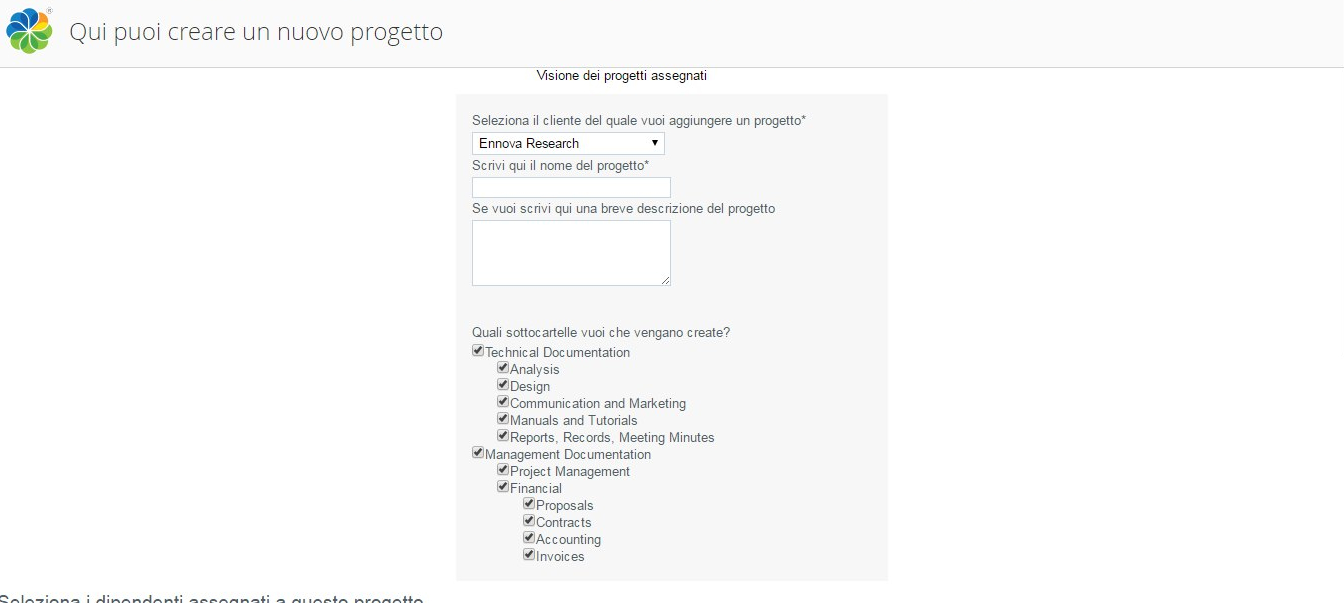
\includegraphics[width=\textwidth]{nuove_immagini/progetti-sopra}
\caption{pagina di inserimento di un nuovo progetto, inserimento dei dati\label{fig:progetti-sopra}}
\end{figure}
\begin{figure}[!ht]
\centering
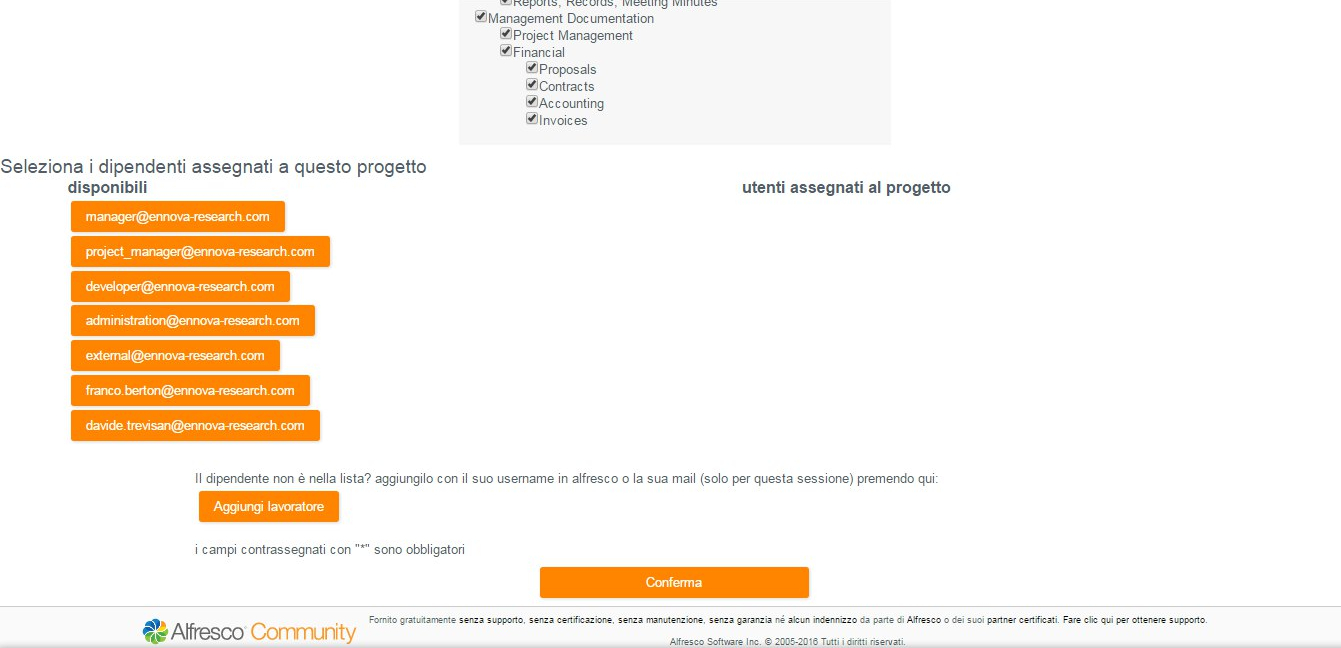
\includegraphics[width=\textwidth]{nuove_immagini/progetti-sotto}
\caption{pagina di inserimento di un nuovo progetto, assegnazione dei lavoratori \label{fig:progetti-sotto}}
\end{figure}
\begin{figure}[!ht]
\centering
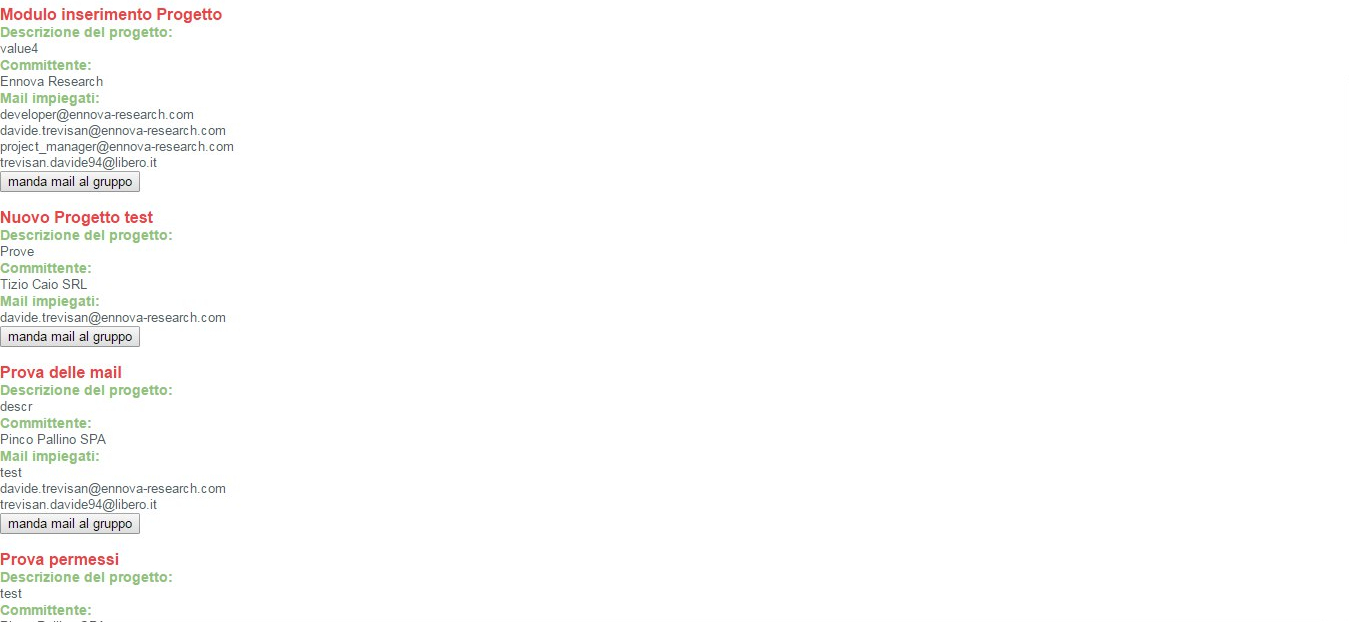
\includegraphics[width=\textwidth]{nuove_immagini/workers}
\caption{pagina di visualizzazione dei progetti \label{fig:workers}}
\end{figure}             % Product Design Freeze e SOP
% !TEX encoding = UTF-8
% !TEX TS-program = pdflatex
% !TEX root = ../tesi.tex
% !TEX spellcheck = it-IT

%**************************************************************
\chapter{Il modulo tema}
\label{cap:modulo-tema}
%**************************************************************

\intro{In questo capitolo verrà esposta l'implementazione e le fasi che hanno portato la creazione del modulo tema}
\section{Scopo del modulo}
Il modulo tema è molto diverso come scopo e implementazione rispetto ai due precedentemente presentati: infatti questo modulo si basa sull'archetipo Share AMP e si pone come scopo non quello di aggiungere nuove funzionalità, ma quello di realizzare un tema gradevole e moderno, che vada ad aggiungersi a quello già presente nel \gls{KMS} aziendale. La difficoltà maggiore di questo modulo è stata quindi quella di dover far convivere i due temi custom e implementare una soluzione che fosse facilmente manutenibile e che inoltre permettesse anche il cambiamento del tema con la difficoltà minore possibile.\\
Era desiderabile, ma non è stato possibile realizzarlo, che ogni utente potesse scegliere un tema diverso.
\section{Realizzazione}
Nella implementazione dei due temi in una unica AMP è stato sfruttato il fatto, che nell'implementazione del tema precedente non era stato tenuto conto, che tutti i file di CSS del tema vengono automaticamente caricati assieme alla pagina share, quindi definendo lo stile con classi e ID (anche nuovi e non del tema) nei file principali del tema e non in file specifici per la pagina come nell'implementazione precedente, è possibile poter cambiare il CSS e le immagini importate e mostrate.
Purtroppo, se si cambia tema, a causa del suo sistema di caching, gli utenti che non hanno effettuato il cambiamento non vedranno sostituito il loro tema fino a un riavvio della componente Share di Alfresco.
\paragraph{}Visto quanto esposto, si è reso necessario un refactoring del modulo tema e dei due moduli, uno che implementa il tema e il login, e l'altro che implementa la funzionalità di recupero password già presenti nel sistema e realizzati precedentemente, per allinearli a quanto prima esposto. Si sono quindi portati tutti i CSS custom nei file del tema, denominato tema Ennova, al fianco del quale si sono implementati i file del nuovo tema, chiamato tema Coral Tree. Si è dovuto quindi togliere dai moduli i riferimenti ai fogli di stile specifici, che altrimenti avrebbero sovrascritto i CSS di tema, e si sono dovuti accorpare i CSS di quei fogli nel tema principale.
\paragraph{} Siccome le modifiche sono avvenute anche riutilizzando il materiale precedente, a seguito si mostrerà solo quanto aggiunto e si trascureranno i file già presenti.
\subsection{File aggiunti nel modulo}
\subsubsection{Diagramma delle cartelle}
Nella figura \ref{fig:cartelle-tema} si illustra in generale quanto è stato prodotto di nuovo per questo modulo. In seguito, nella descrizione di dettaglio, si indicheranno i nomi specifici dei file più importanti che sono stati creati o modificati.
\begin{figure}
\centering
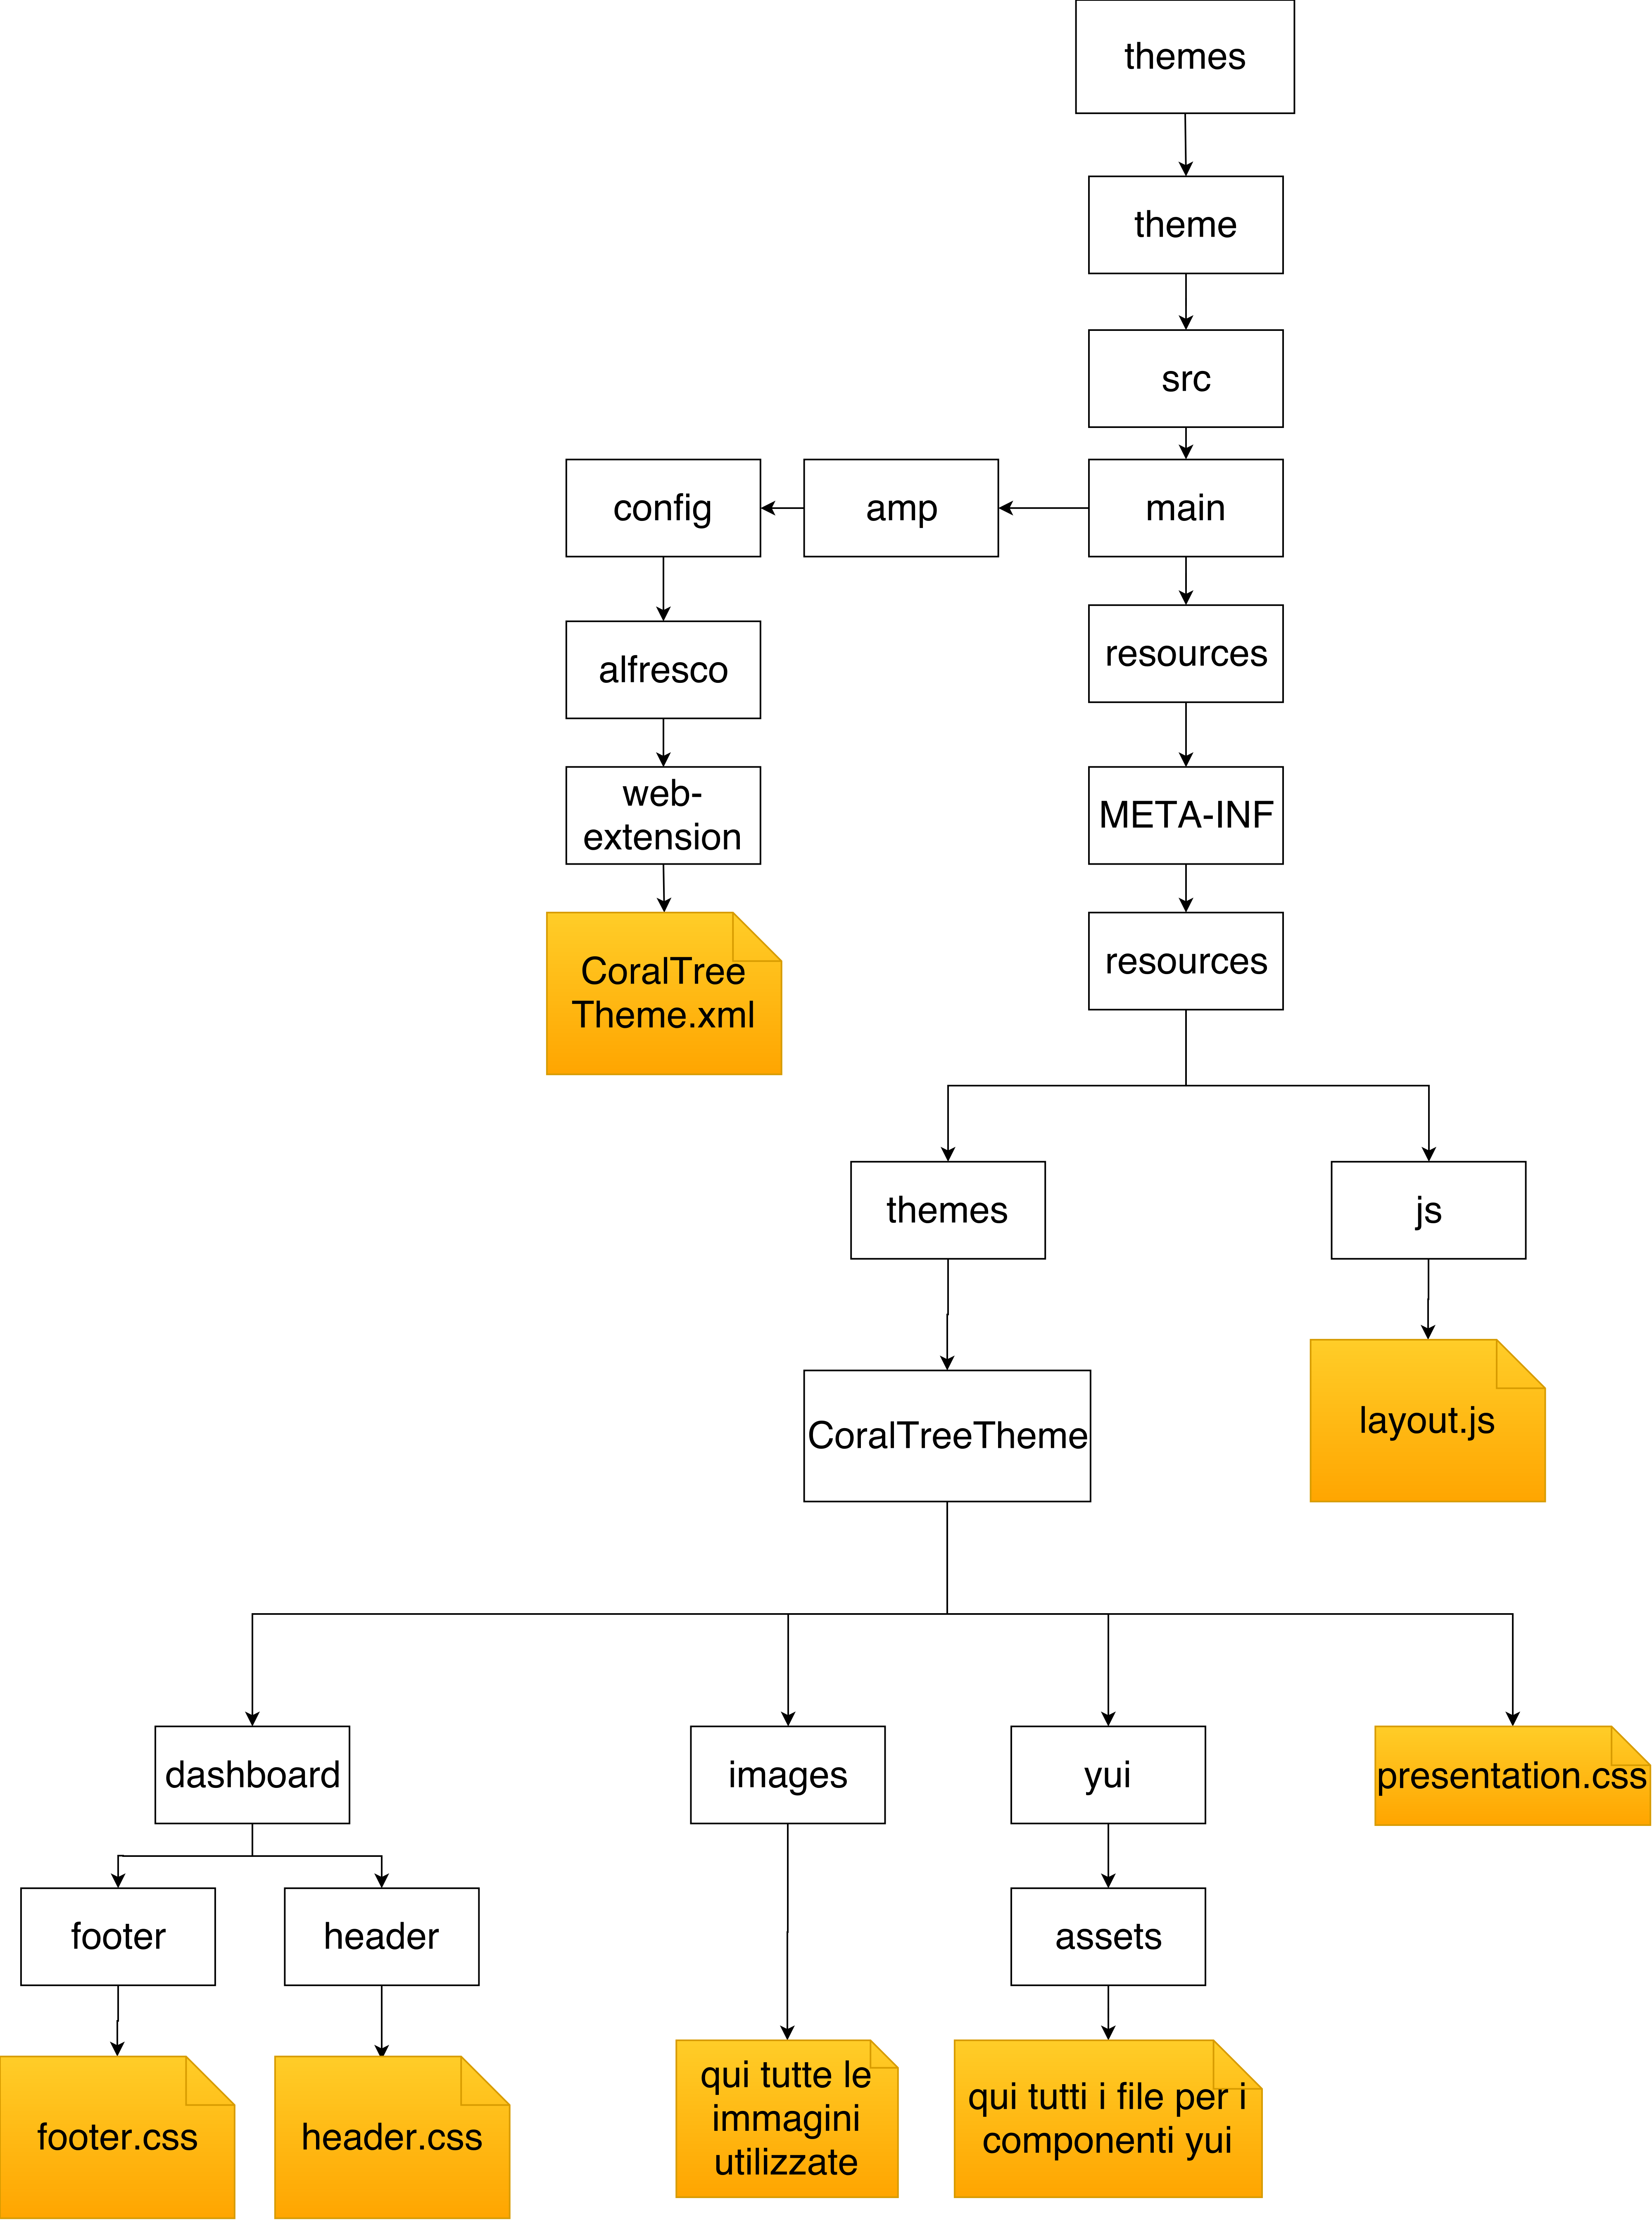
\includegraphics[width=\textwidth]{/diagrammi_cartelle/temifolder.png}
\caption{descrizione generale di quanto creato per il modulo relativo ai temi\label{fig:cartelle-tema}}
\end{figure}
\FloatBarrier
\subsubsection{File di funzionalità}
Per registrare il tema tra quelli di Alfresco stato innanzitutto aggiunto il file CoralTreeTheme.xml, il cui contenuto è riportato nel listato \ref{lst:theme-declaration} che serve a registrare il tema.
\begin{lstlisting}[language=XML, caption=XML della dichiarazione del tema, label=lst:theme-declaration]
<?xml version='1.0' encoding='UTF-8'?>
<theme>
    <title>Coral Tree Theme</title>
    <title-id>theme.CoralTreeTheme</title-id>
    <css-tokens>
        <less-variables>
            <!-- Only for Alfresco 5.x onwards and latest Aikau version -->
        </less-variables>
    </css-tokens>
</theme>
\end{lstlisting}
Innanzitutto è stato creato aggiornato il file layout.js, che si occupa di gestire il tema selezionato, e il cui testo integrale è riportato nel listato \ref{code-layout}. Come si può vedere, si controlla nelle costanti di Alfresco quale è il tema attivo e in base a quello si inietta il codice per importare i file corretti.
\begin{lstlisting}[language=JavaScript, caption=codice di layout.js, label=code-layout]
$( window ).load(function() {
    /** CoralTreeTheme **/
    if (Alfresco.constants.THEME == "CoralTreeTheme") {
        document.getElementById("HEADER_SEARCHBOX_FORM_FIELD").setAttribute("placeholder","Chi cerca, trova!");
        var arrayLink = ['/share/res/themes/CoralTreeTheme/dashboard/header/header.css', '/share/res/themes/CoralTreeTheme/dashboard/footer/footer.css'];
        for (i = 0; i < arrayLink.length; i++) {
            var link = document.createElement("link");
            link.rel = 'stylesheet';
            link.type = 'text/css';
            link.href = arrayLink[i];
            document.querySelector("head").appendChild(link);
        }
        var arrayScript = ['/share/res/js/CoralTreeTheme/dashboard/header/header.js', '/share/res/js/CoralTreeTheme/dashboard/footer/footer.js'];
        for (i = 0; i < arrayScript.length; i++) {
            var script = document.createElement("script");
            script.type= "text/javascript";
            script.src = arrayScript[i];
            document.querySelector("head").appendChild(script);
        }
        $(".yui-skin-CoralTreeTheme").css({"display":"block"});
    } else if (Alfresco.constants.THEME == "ennovaTheme") {
        var arrayLink = ['/share/res/themes/ennovaTheme/dashboard/header/header.css', '/share/res/themes/ennovaTheme/dashboard/footer/footer.css'];
        for (i = 0; i < arrayLink.length; i++) {
            var link = document.createElement("link");
            link.rel = 'stylesheet';
            link.type = 'text/css';
            link.href = arrayLink[i];
            document.querySelector("head").appendChild(link);
        }
        var arrayScript = ['/share/res/js/ennovaTheme/dashboard/header/header.js', '/share/res/js/ennovaTheme/dashboard/footer/footer.js'];
        for (i = 0; i < arrayScript.length; i++) {
            var script = document.createElement("script");
            script.type= "text/javascript";
            script.src = arrayScript[i];
            document.querySelector("head").appendChild(script);
        }
        $(".yui-skin-ennovaTheme").css({"display":"block"});
    }
});
\end{lstlisting}
\subsubsection{File di stile}
Per realizzare il tema si sono seguite le linee guida di Alfresco, che dicono di copiare i file di uno dei tema base e di lavorare su quelli, aggiungendo gli stili desiderati. Si hanno quindi:
\begin{itemize}
\item \texttt{footer.css}, che contiene il CSS specifico per il footer
\item \texttt{header.css}, che contiene il CSS specifico per l'header.
\item la cartella \texttt{images}, che contiene le immagini che sono usate dal tema
\item \texttt{presentation.css} che è il CSS principale del tema
\item la cartella \texttt{assets}, che contiene il CSS e i file necessari per i componenti \gls{YUI} utilizzati da Alfresco
\end{itemize}
\section{Aspetto estetico}
Per il lato estetico ci si è ancora una volta dovuti rivolgere al team di grafici che lavorano presso l'azienda per ottenere un mockup. Sono stati utilizzati quelli già prodotti nel passato al momento della presentazione del progetto e della creazione dei primi moduli.
\subsection{Risultati raggiunti}
Nella figura \ref{fig:login} si può vedere l'aspetto della pagina di inserimento di login, mentre nella figura \ref{fig:forgotpwd} si può vedere la pagina per la password dimenticata. Nelle figure \ref{fig:old-home} e \ref{fig:home} si può vedere il confronto tra il tema predefinito di Alfresco e quanto prodotto relativamente alla schermata dell'utente, nelle figure \ref{fig:old-site-home} e \ref{fig:site-home} relativamente alla home page di un sito e nelle figure \ref{fig:old-raccolta} e \ref{fig:raccolta} relativamente alla raccolta dei documenti. Si noti come l'intento sia stato quello di creare un aspetto più moderno con colori più accesi e vivaci rispetto alla normale interfaccia di Alfresco, molto arretrata.
\begin{figure}[!ht]
\centering
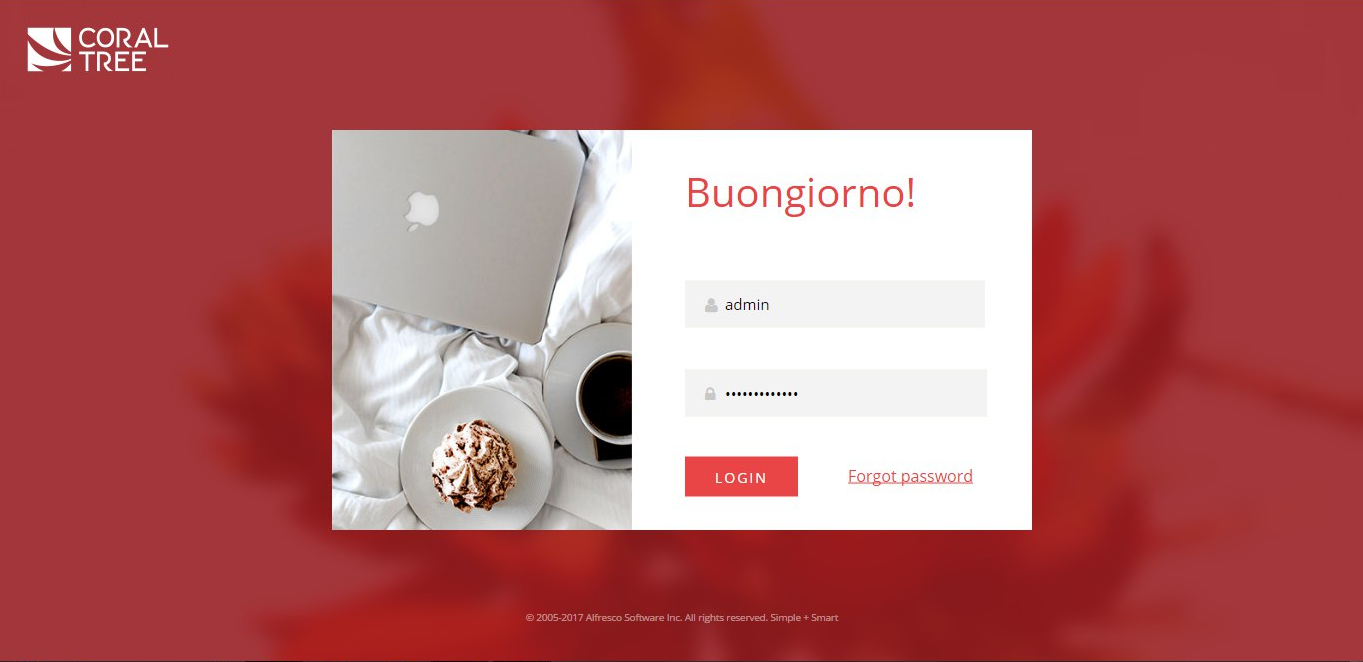
\includegraphics[width=\textwidth]{nuove_immagini/login}
\caption{pagina di login\label{fig:login}}
\end{figure}
\begin{figure}[!ht]
\centering
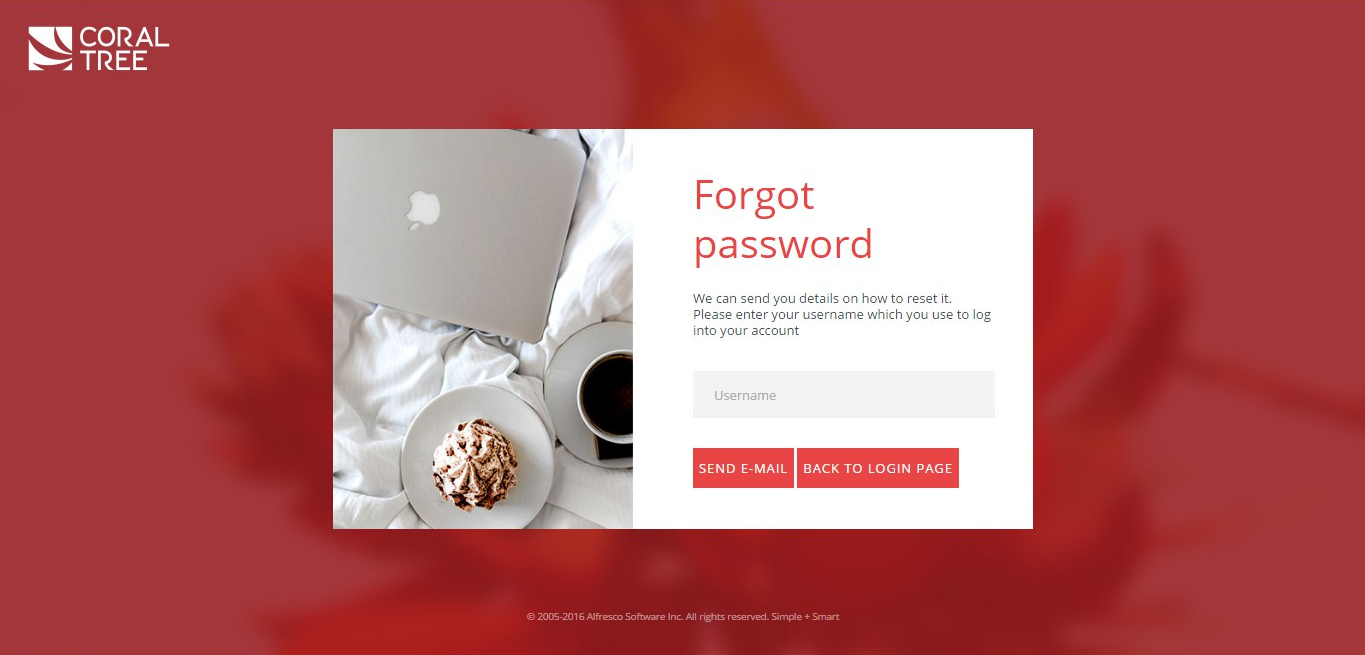
\includegraphics[width=\textwidth]{nuove_immagini/forgotpwd}
\caption{pagina per la password dimenticata\label{fig:forgotpwd}}
\end{figure}
\begin{figure}[!ht]
\centering
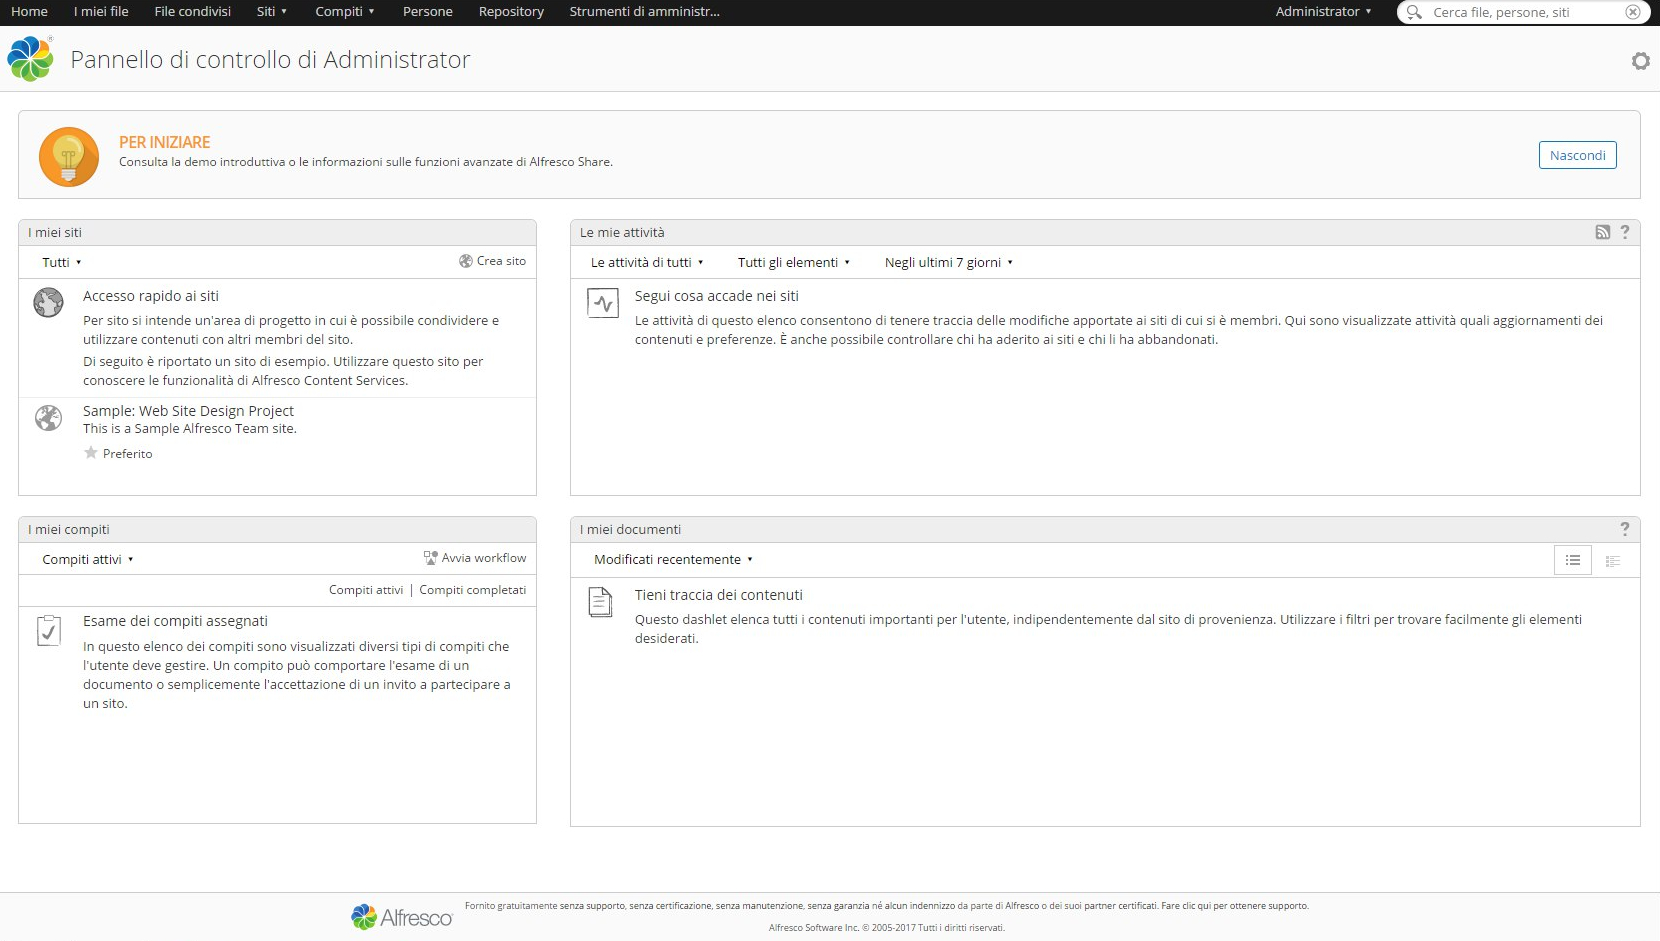
\includegraphics[width=\textwidth]{nuove_immagini/old-home}
\caption{home page predefinita di Alfresco \label{fig:old-home}}
\end{figure}
\begin{figure}[!ht]
\centering
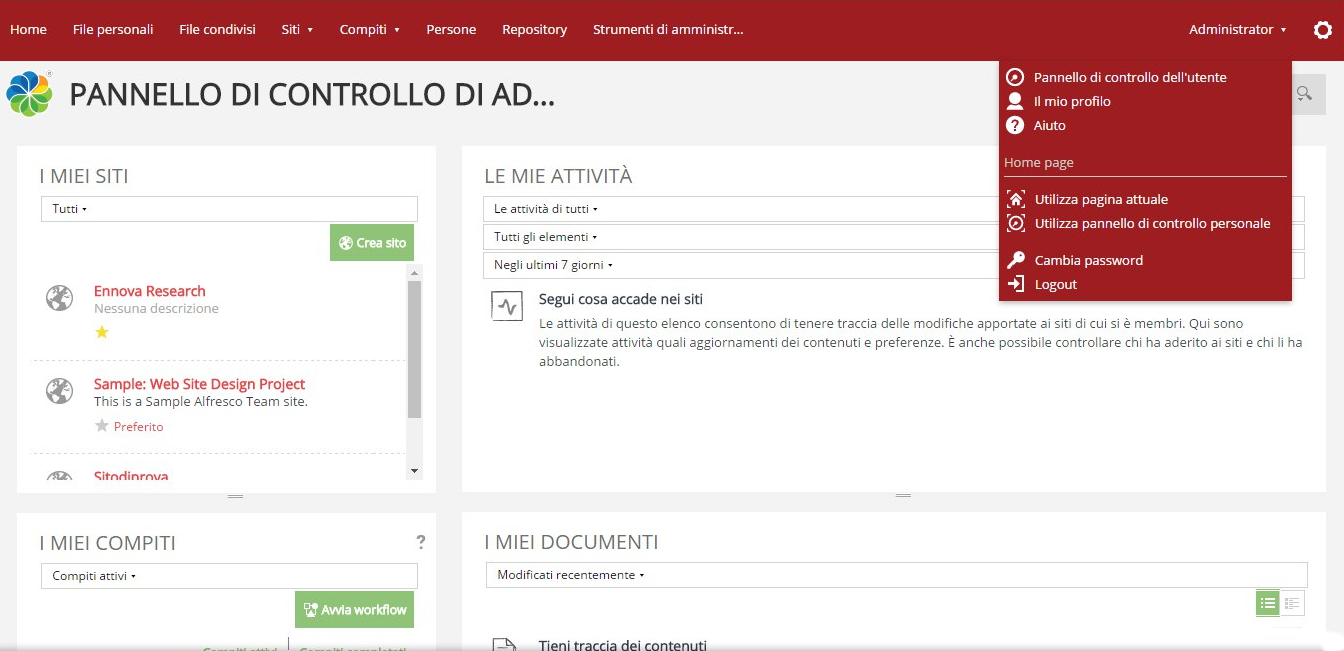
\includegraphics[width=\textwidth]{nuove_immagini/home}
\caption{nuovo aspetto della home page \label{fig:home}}
\end{figure}
\begin{figure}[!ht]
\centering
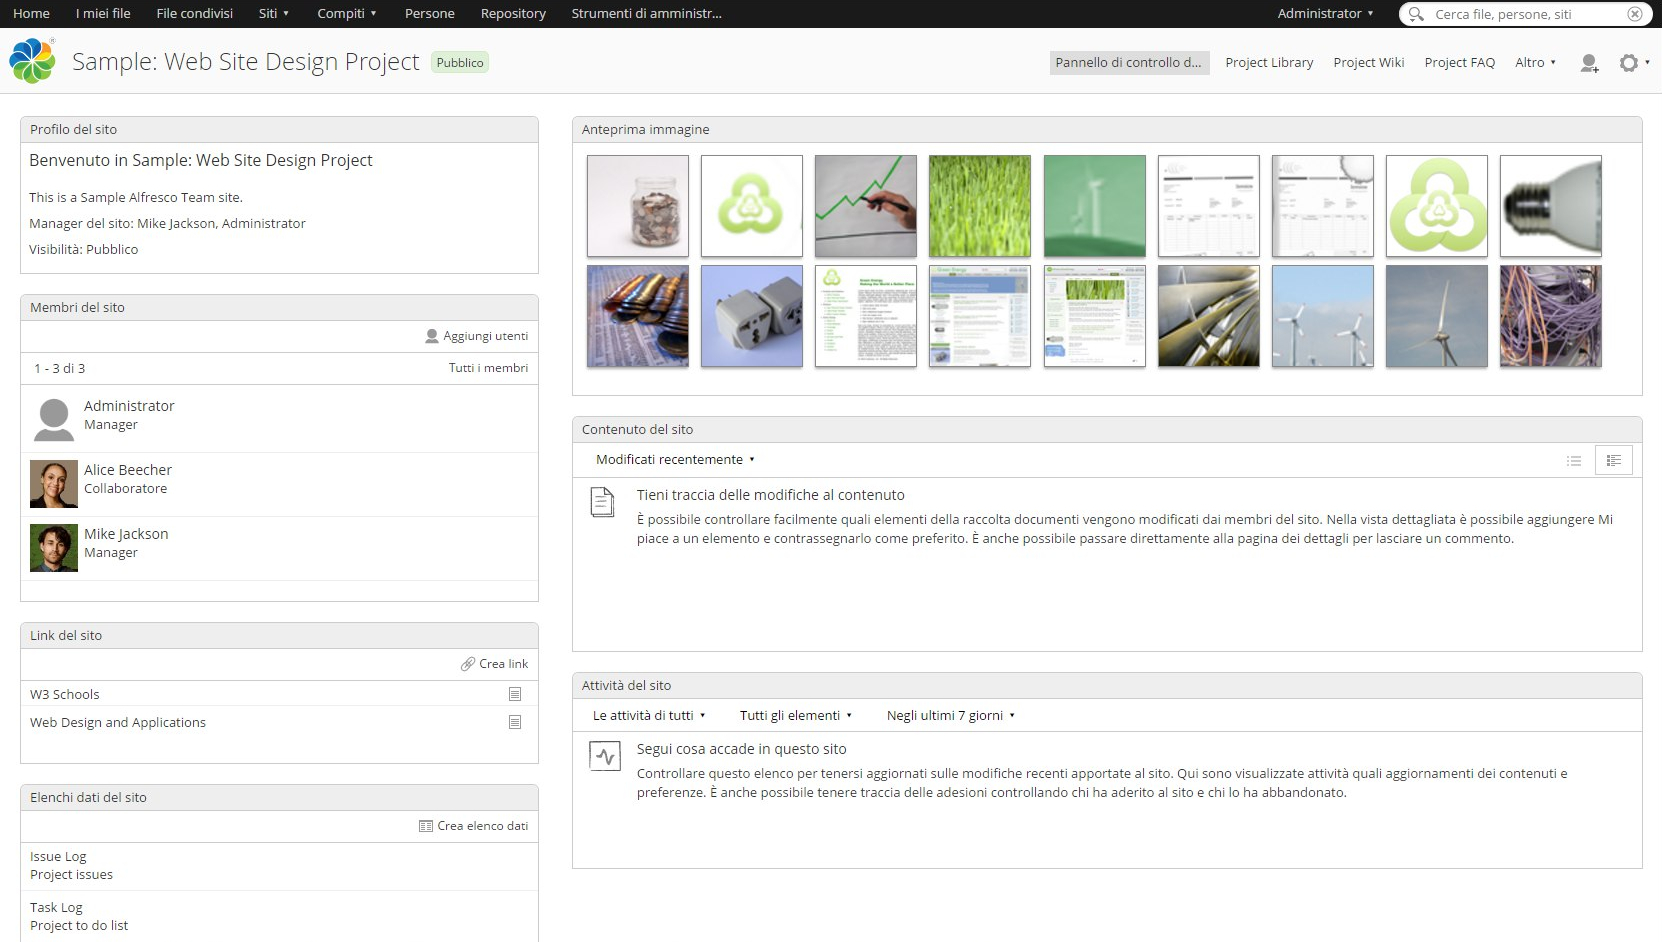
\includegraphics[width=\textwidth]{nuove_immagini/old-site-home}
\caption{pagina principale di un sito di Alfresco, tema predefinito \label{fig:old-site-home}}
\end{figure}
\begin{figure}[!ht]
\centering
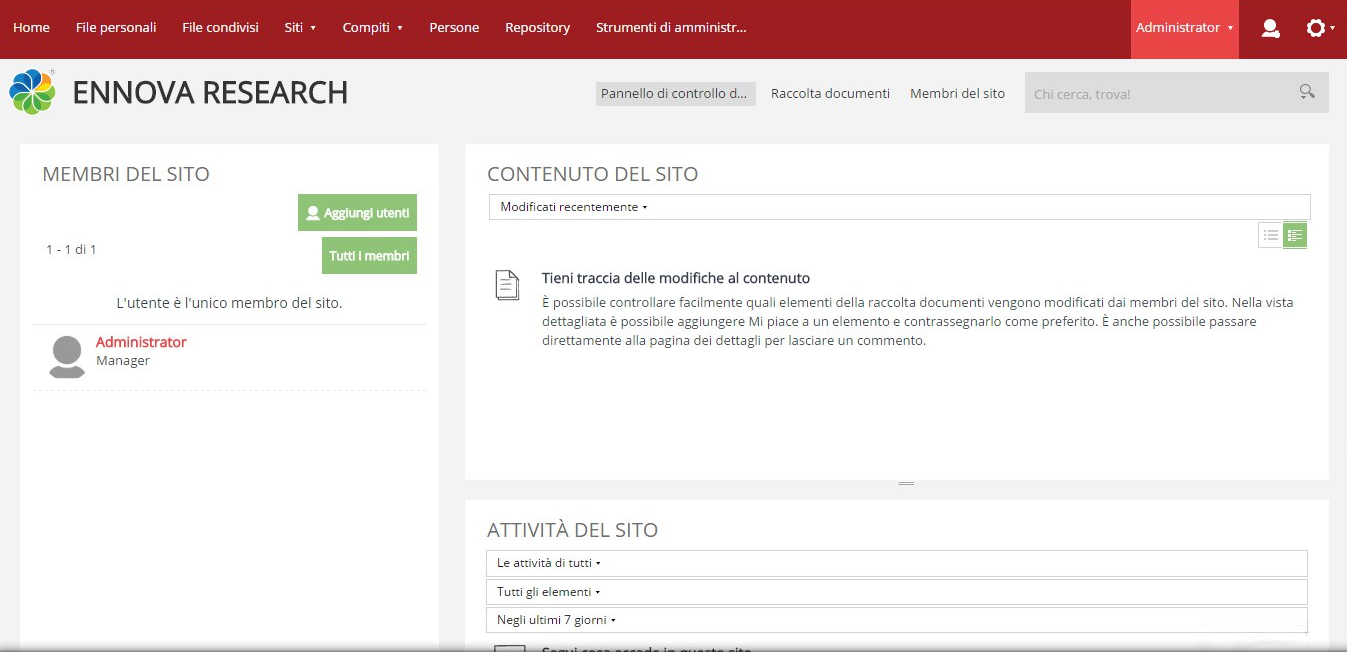
\includegraphics[width=\textwidth]{nuove_immagini/site-home}
\caption{pagina principale di un sito di Alfresco, nuovo aspetto \label{fig:site-home}}
\end{figure}
\begin{figure}[!ht]
\centering
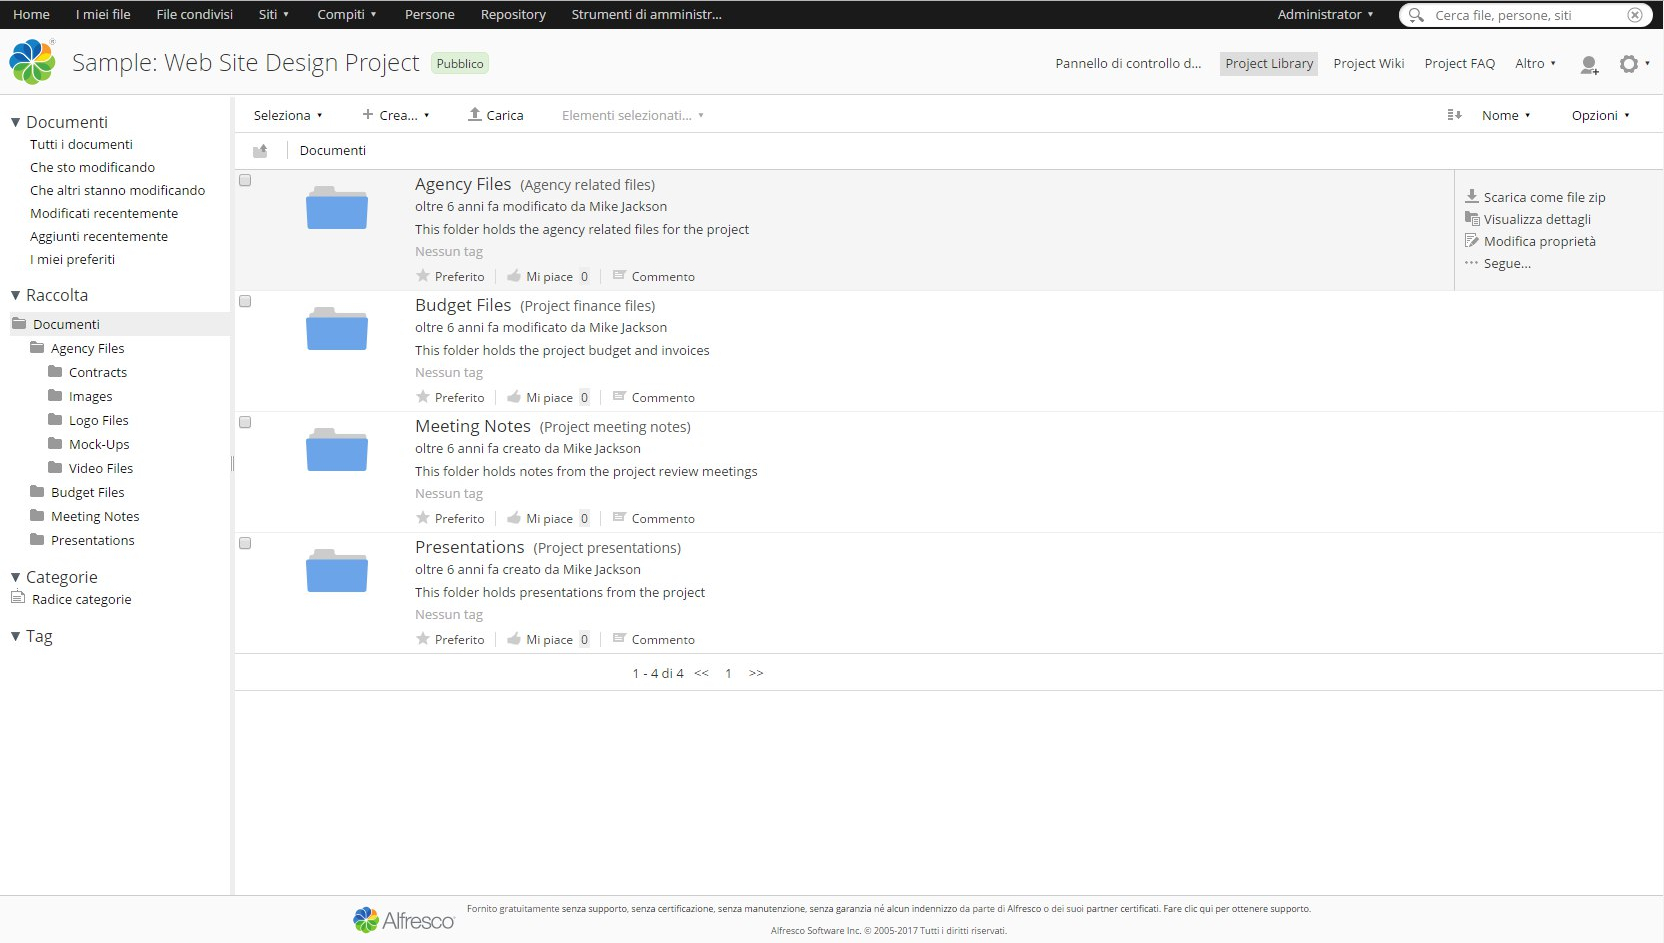
\includegraphics[width=\textwidth]{nuove_immagini/old-raccolta}
\caption{raccolta documenti predefinita di Alfresco \label{fig:old-raccolta}}
\end{figure}
\begin{figure}[!ht]
\centering
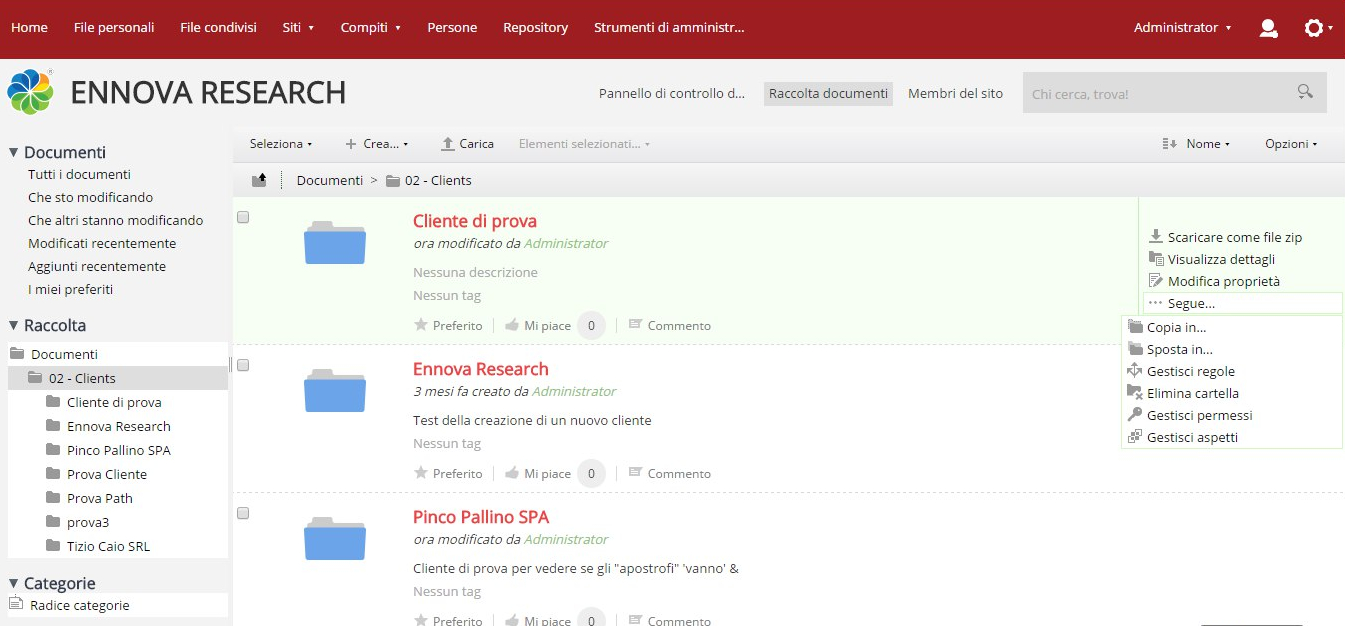
\includegraphics[width=\textwidth]{nuove_immagini/raccolta}
\caption{nuovo aspetto della raccolta documenti \label{fig:raccolta}}
\end{figure}         % Aggiuntivo per il tema
% !TEX encoding = UTF-8
% !TEX TS-program = pdflatex
% !TEX root = ../tesi.tex
% !TEX spellcheck = it-IT

%**************************************************************
%**************************************************************
%
%**************************************************************
%\section{Consuntivo finale}
%
%**************************************************************
%\section{Raggiungimento degli obiettivi}
%
%**************************************************************
%\section{Conoscenze acquisite}
%
%**************************************************************
%\section{Valutazione personale}
\chapter{Conclusioni}
\label{cap:conclusioni}

Il tirocinio formativo si è svolto secondo i tempi inizialmente concordati,
 non ci sono stati ritardi evidenti e i risultati ottenuti hanno pienamente
soddisfatto le aspettative dell’azienda, dimostrando l'effettiva possibilità di costruire in 
Alfresco una piattaforma evoluta e complessa per la gestione dei progetti e dei clienti. È stata
espressa infatti da parte dell’azienda la volontà di proseguire allo sviluppo e all’integrazione
del sistema in produzione e sono previste ulteriori espansioni del sistema in futuro, per fornire un sistema completo e vendibile come scopo ultimo.
\section{Prospettive future}
Il sistema, ora in produzione, punta ad essere espanso con nuove funzionalità per la gestione dei progetti e dei loro processi, al fine di garantire una gestione migliore degli stessi e dei loro costi, oltre alla volontà di integrare in Alfresco elementi social.
La piattaforma dei clienti in futuro verrà integrata con i progetti ad essi relativi e, come fine ultimo, verrà dotata di ulteriori funzionalità allo stato attuale non concretamente possibili, come ad esempio la creazione di fatture intelligenti che tengano conto di quanto rendicontato in un ipotetico futuro modulo progetti più evoluto.
\section{Difficoltà e limiti riscontrati}
Il progetto è stato svolto senza particolari intoppi, tuttavia vi sono state alcune difficoltà, sia di natura tecnica che di altro genere, di seguito riportate:
\begin{itemize}
\item la completa inesperienza sul sistema Alfresco, sul suo funzionamento e sulle tecnologie che utilizza, che, anche se mitigata dall'aiuto ricevuto, ha comportato tempi di apprendimento lunghi, data anche la sua complessa architettura.
Ciò ha portato infatti a scelte di cui non sono completamente soddisfatto per quanto riguarda l'implementazione di alcune funzionalità, che, con l'esperienza acquisita anche solo alla fine dello stage, sarebbe stata molto diversa;
\item i tempi piuttosto lunghi della compilazione e lancio dell'All-in-one SDK, dato che il codice Java non gode del RAD, quindi ogni aggiunta, prima di poter essere provata nell'SDK, doveva essere preceduta dal rilancio dell'SDK, che nel dispositivo fornito dall'azienda poteva anche durare più di 30 minuti;
\item l'iniziale assenza di una piattaforma dove poter effettivamente provare i moduli prima di portarli nell'ambiente di produzione, che è stata opportunamente creata sempre nell'ambito dello stage.
\end{itemize}
\section{Considerazioni personali}
Dal punto di vista formativo l'esperienza è stata sicuramente soddisfacente, in quanto mi ha permesso di avere un contatto con un'azienda che opera nel settore informatico ed avere esperienza diretta di come si lavora in quest'ambiente; sono restato molto soddisfatto del clima e dell'accoglienza che mi è stata riservata nell'azienda, oltre all'opportunità che mi è stata da loro concessa di poter continuare a lavorare presso di loro.
È stata una esperienza estremamente interessante e degna conclusione del mio percorso di studi.             % Conclusioni
\appendix                               
% !TEX encoding = UTF-8
% !TEX TS-program = pdflatex
% !TEX root = ../tesi.tex
% !TEX spellcheck = it-IT

%**************************************************************
%S\chapter{Appendice}
%**************************************************************

%\epigraph{Citazione}{Autore della citazione}



             % Appendice A

%**************************************************************
% Materiale finale
%**************************************************************
\backmatter
\printglossaries
% !TEX encoding = UTF-8
% !TEX TS-program = pdflatex
% !TEX root = ../tesi.tex
% !TEX spellcheck = it-IT

%**************************************************************
% Bibliografia
%**************************************************************

\cleardoublepage
\chapter{Bibliografia}

\nocite{*}
%\printbibliography

\bibbycategory % equivale a dare un \printbibliography per ogni categoria


\end{document}